\documentclass{beamer}

\usepackage{listings}
\usetheme{Warsaw}
\setbeamertemplate{footline}[frame number]
\usepackage[latin1]{inputenc}
\usepackage{verbatim}
\usepackage{color}
\usepackage{amsmath}
\usepackage{amsfonts}
\usepackage{ifthen}

\lstset{language=python,
  basicstyle=\ttfamily,
  keywordstyle=\color{blue}\ttfamily,
breaklines=true}

\def\xcolorversion{2.00}
\def\xkeyvalversion{1.8}
\usepackage[version=0.96]{pgf}
\usepackage{tikz}
\usetikzlibrary{arrows, positioning}

\begin{document}
\begin{frame}
  \tableofcontents
\end{frame}

\section{Introduction}
\tableofcontents[sectionstyle=show/shaded]
\begin{frame}
  \begin{center}
    \Large{Machine learning}
  \end{center}
\end{frame}

% TODO ? graph with pictures of digits on the x-axis and their corresponding digit
% on the y-axis

\begin{frame}
  \begin{center}
    \begin{tikzpicture}[]

      % horizontal axis
      \draw[->] (0,0) -- (5,0) node[anchor=north] {};
      \draw   (0.5,0) node[anchor=north] {
\includegraphics[scale=0.2]{./pictures/0.png}}
      (1.0,0) node[anchor=north] {
\includegraphics[scale=0.3]{./pictures/1.png}}
      (1.5,0) node[anchor=north] {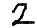
\includegraphics[scale=0.3]{./pictures/2.png}}
      (2.0,0) node[anchor=north] {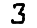
\includegraphics[scale=0.3]{./pictures/3.png}}
      (2.5,0) node[anchor=north] {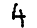
\includegraphics[scale=0.3]{./pictures/4.png}}
      (3.0,0) node[anchor=north] {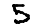
\includegraphics[scale=0.3]{./pictures/5.png}}
      (3.5,0) node[anchor=north] {
\includegraphics[scale=0.3]{./pictures/6.png}}
      (4.0,0) node[anchor=north] {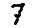
\includegraphics[scale=0.3]{./pictures/7.png}}
      (4.5,0) node[anchor=north] {
\includegraphics[scale=0.3]{./pictures/8.png}}
      (5.0,0) node[anchor=north] {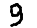
\includegraphics[scale=0.3]{./pictures/9.png}};

      % horizontal axis
      \draw[->] (0,0) -- (0,5) node[anchor=north] {};
      \draw (0,0.5) node[anchor=east] {0}
      (0,1.0) node[anchor=east] {1}
      (0,1.5) node[anchor=east] {2}
      (0,2.0) node[anchor=east] {3}
      (0,2.5) node[anchor=east] {4}
      (0,3.0) node[anchor=east] {5}
      (0,3.5) node[anchor=east] {6}
      (0,4.0) node[anchor=east] {7}
      (0,4.5) node[anchor=east] {8};
      (0,5.0) node[anchor=east] {9};

      \node (?) at (2.5, 2.5) {?};

    \end{tikzpicture}
  \end{center}
\end{frame}

\begin{frame}
  \begin{center}
  \begin{tikzpicture}[shorten >=1pt,->,draw=black!50, node distance=2.5cm]
    \tikzstyle{every pin edge}=[<-,shorten <=1pt]
    \tikzstyle{neuron}=[circle,draw,minimum size=17pt,inner sep=0pt]

    % input layer nodes
    \foreach \y in {1,...,4}
    \node[neuron, pin=left:$x\y$] (I-\y) at (0,-\y) {};

    % hidden layer nodes
    \foreach \y in {1,...,5}
    \path[yshift=0.5cm]
    node[neuron] (H-\y) at (2.5,-\y) {};

    % output layer node
    \foreach \y in {1,2}
    \path[yshift=-1cm]
    node[neuron,pin={[pin edge={->}]right:$o\y$}] (O-\y) at (4.5,-\y) {};

    % Connect every node in the input layer with every node in the
    % hidden layer.
    \foreach \src in {1,...,4}
    \foreach \dst in {1,...,5}
    \path (I-\src) edge (H-\dst);

    % Connect every node in the hidden layer with the output layer
    \foreach \src in {1,...,5}
    \foreach \dst in {1,2}
    \path (H-\src) edge (O-\dst);
  \end{tikzpicture}
  \end{center}
\end{frame}

%\begin{frame}
  %\frametitle{Prerequisites}
  %\begin{itemize}
    %\item Derivative of composed functions
    %\item Matrix multiplication
    %\item Some python
  %\end{itemize}
%\end{frame}

%\begin{frame}
  %\frametitle{Derivative of composed functions}
  %\begin{equation*}
    %\begin{split}
      %f(g(h(x)))' & = f'(g(h(x))) g'(h(x)) h'(x) \\
      %& = \frac{d f}{d g} \cdot \frac{d g}{d h} \cdot \frac{d h}{d x}
    %\end{split}
  %\end{equation*}
%\end{frame}

%\begin{frame}
  %\frametitle{Matrix multiplication}
  %$
  %\begin{array}{cc}
    %&
    %\left(
      %\begin{matrix}
        %b_{11} & \ldots & b_{12} \\
        %\vdots & \ddots & \vdots \\
        %b_{n1} & \ldots & b_{np}
      %\end{matrix}
    %\right) \\
    %&\\
    %\left(
      %\begin{matrix}
        %a_{11} & \ldots & a_{1n} \\
        %\vdots & \ddots & \vdots \\
        %a_{m1} & \ldots & a_{mn}
      %\end{matrix}
    %\right) & \left(
      %\begin{matrix}
        %c_{11} & \ldots & c_{1p} \\
        %\vdots & \ddots & \vdots \\
        %c_{m1} & \ldots & c_{mp}
      %\end{matrix}
    %\right)
  %\end{array}
  %\qquad c_{ij} = \displaystyle\sum_{k=1}^n{a_{ik} b_{kj}}
  %$
%\end{frame}

%\begin{frame}[fragile]
  %\frametitle{Python}
  %\begin{block}{}
    %\begin{lstlisting}
%def foo(x):
    %l1 = [1, 2, 3, 4]
    %l2 = [5, 6, 7, 8]
    %for elt in l:
        %print(x + elt)
    %for i in range(len(l1)):
        %print(x * l1[i] + l2[i])
    %\end{lstlisting}
  %\end{block}
%\end{frame}

%\begin{frame}[fragile]
  %\frametitle{Numpy}
  %\begin{block}{}
    %\begin{lstlisting}
%from numpy import matrix

%a = matrix([
    %[1, 2, 3],
    %[4, 5, 6]]
%b = matrix([
    %[6, 5],
    %[4, 3],
    %[2, 1]])
%c = a * b
    %\end{lstlisting}
  %\end{block}
%\end{frame}


\section{Binary classification}
\tableofcontents[sectionstyle=show/shaded]
\begin{frame}
\frametitle{Binary classifier}
\begin{tikzpicture}[->,>=stealth',shorten >=1pt,auto,node distance=3cm,
  thick,main node/.style={circle,fill=blue!20,draw,font=\sffamily\Large\bfseries}]
%
  \node[style={font=\sffamily\Large\bfseries}] (1)
  {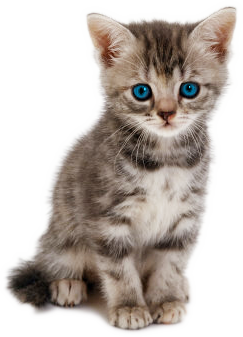
\includegraphics[scale=0.14]{./pictures/kitten.png}};
  \onslide<3>{
    \node[main node] (2) [right of=1]
    {$h(\raisebox{-0.2cm}{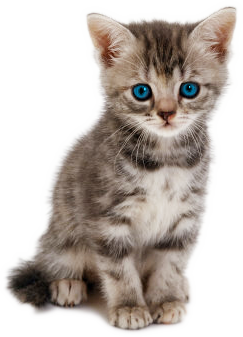
\includegraphics[scale=0.06]{./pictures/kitten.png}})$};
    \node[main node] (3) [below right of=2] {$0$};
    \node[main node] (4) [above right of=2] {$1$};
  %
    \path[every node/.style={font=\sffamily\small}]
       (1) edge node [right] {} (2)
       (2) edge node [right] {} (3)
       (2) edge node [right] {} (4);
     }
  \onslide<2-3>{
    \node (inA) [right=0.5cm of 4] {$\in A$};
    \node (notinA) [right=0.5cm of 3] {$\notin A$};
  }
\end{tikzpicture}
\end{frame}

\begin{frame}
  \begin{center}
    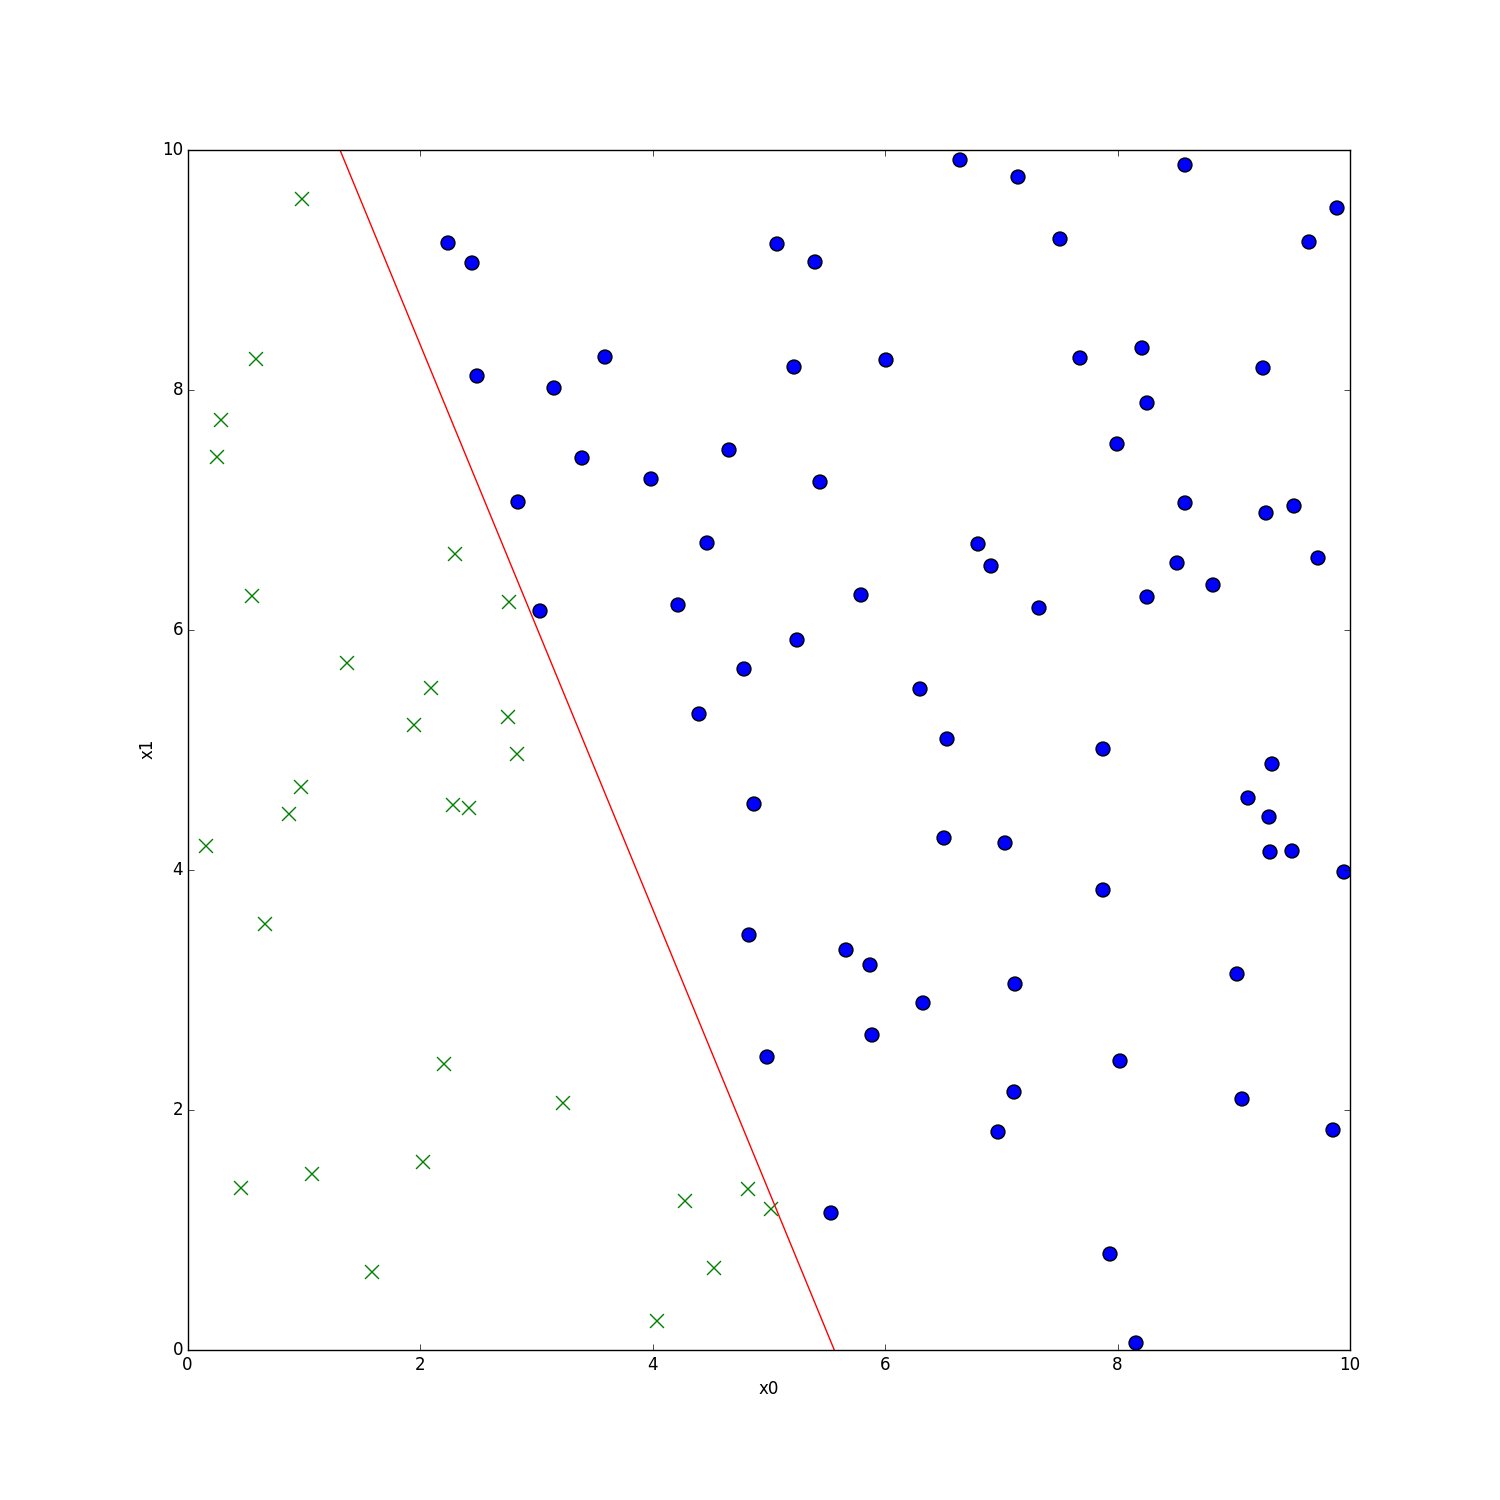
\includegraphics[scale=0.2]{./pictures/logreg_db078.png}
  \end{center}
\end{frame}

\begin{frame}
  \frametitle{Hypothesis function}
  $h_w:
  \left \{
    \begin{array}{ccc}
      \{0, 1\}^n & \to & \mathbb{N} \\
      (x_1, \ldots, x_{n}) & \mapsto &
      \displaystyle\sum_{i=1}^n{w_i x_i} \\
    \end{array}
  \right.$
\end{frame}

\begin{frame}[fragile]
  \begin{block}{Hypothesis function}
      \begin{lstlisting}
def h(x, w):
    sum = 0
    for i in range(len(x)):
        sum += w[i] * x[i]
    return sum
      \end{lstlisting}
  \end{block}
\end{frame}

\begin{frame}[fragile]
  \frametitle{Notation}
  $
  \begin{array}{cc}
    \onslide<2>{
      &
      \left(
        \begin{matrix}
          x_1 \\
          \vdots \\
          x_n
        \end{matrix}
      \right) \\}
    &\\
    \onslide<2>{\left(
      \begin{matrix}
        w_1 & \ldots & w_{n}
      \end{matrix}
    \right)} & {\left( \displaystyle\sum_{i = 1}^n{w_i x_i} \right)}
  \end{array}
  $
\end{frame}

\begin{frame}[fragile]
  \hspace{2em}
  \begin{block}{Hypothesis}
    \begin{lstlisting}
def h(x, w):
    return transpose(w) * x
    \end{lstlisting}
  \end{block}
\end{frame}

\begin{frame}
  \frametitle{Step function}
  To force the output of $h$ to be in $\{0, 1\}$, we use the Heaviside step function:
  \vspace{1cm}

  $g:
  \left \{
    \begin{array}{ccc}
      \mathbb{N} & \to & \{0, 1\} \\
      x & \mapsto &
      \begin{array}{cc}
        1 & $if $ x >= 0 \\
        0 & $otherwise$
      \end{array}
    \end{array}
  \right.$
\end{frame}

\begin{frame}
  \begin{center}
    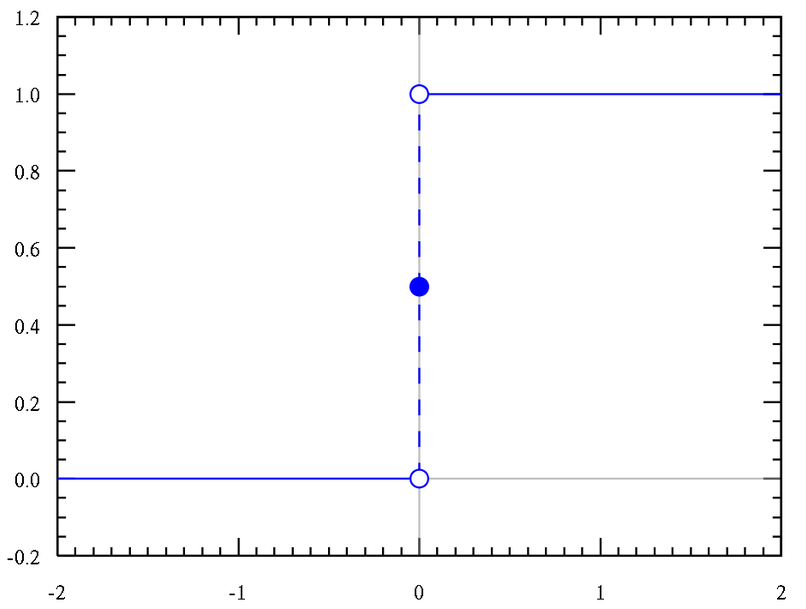
\includegraphics[scale=0.4]{./pictures/step_function.png}
  \end{center}
\end{frame}

\begin{frame}[fragile]
  \begin{block}{Step function}
      \begin{lstlisting}
def g(x):
    if x >= 0:
        return 1
    else:
        return 0
      \end{lstlisting}
  \end{block}
\end{frame}

\begin{frame}[fragile]
  \begin{block}{Step function}
      \begin{lstlisting}
def g(x):
    return x >= 0
      \end{lstlisting}
  \end{block}
\end{frame}


\begin{frame}
  \frametitle{}
  $h_w:
  \left \{
    \begin{array}{ccc}
      \{0, 1\}^n & \to & \{0, 1\} \\
      x & \mapsto &
      g(w^T x) \\
    \end{array}
  \right.$
\end{frame}

\begin{frame}[fragile]
  \begin{block}{}
      \begin{lstlisting}
def h(x, w):
    return g(transpose(w) * x)
      \end{lstlisting}
  \end{block}
\end{frame}

\begin{frame}
  \frametitle{Example}
  image:
  \nolinebreak
  $
  \left(
    \begin{matrix}
      0 & 0 & \colorbox{gray}{1} & \colorbox{gray}{1} & 0 & 0 \\
      0 & \colorbox{gray}{1} & 0 & 0 & \colorbox{gray}{1} & 0 \\
      0 & \colorbox{gray}{1} & 0 & 0 & 0 & 0 \\
      0 & \colorbox{gray}{1} & 0 & 0 & 0 & 0 \\
      0 & \colorbox{gray}{1} & 0 & 0 & \colorbox{gray}{1} & 0 \\
      0 & 0 & \colorbox{gray}{1} & \colorbox{gray}{1} & 0 & 0
    \end{matrix}
  \right)
  $
  \newline
  weights:
  \nolinebreak
  $
  \only<1>{
    \left(
      \begin{matrix}
        w0 & w1 & w2 & w3 & w4 & w5 \\
        w6 & w7 & w8 & w9 & w10 & w11 \\
        w12 & w13 & w14 & w15 & w16 & w17 \\
        w18 & w19 & w20 & w21 & w22 & w23 \\
        w24 & w25 & w26 & w27 & w28 & w29 \\
        w30 & w31 & w32 & w33 & w34 & w35
      \end{matrix}
    \right)
  }
  \only<2>{
    \left(
    \begin{matrix}
      0 & 0 & \colorbox{gray}{1} & \colorbox{gray}{1} & 0 & 0 \\
      0 & \colorbox{gray}{1} & 0 & 0 & \colorbox{gray}{1} & 0 \\
      0 & \colorbox{gray}{1} & 0 & 0 & 0 & 0 \\
      0 & \colorbox{gray}{1} & 0 & 0 & 0 & 0 \\
      0 & \colorbox{gray}{1} & 0 & 0 & \colorbox{gray}{1} & 0 \\
      0 & 0 & \colorbox{gray}{1} & \colorbox{gray}{1} & 0 & 0
    \end{matrix}
    \right)
  }
  \only<3>{
    \left(
    \begin{matrix}
      -1 & -1 & \colorbox{gray}{1} & \colorbox{gray}{1} & -1 & -1 \\
      -1 & \colorbox{gray}{1} & -1 & -1 & \colorbox{gray}{1} & -1 \\
      -1 & \colorbox{gray}{1} & -1 & -1 & -1 & -1 \\
      -1 & \colorbox{gray}{1} & -1 & -1 & -1 & -1 \\
      -1 & \colorbox{gray}{1} & -1 & -1 & \colorbox{gray}{1} & -1 \\
      -1 & -1 & \colorbox{gray}{1} & \colorbox{gray}{1} & -1 & -1
    \end{matrix}
    \right)
  }
  $
\end{frame}

\begin{frame}
  \begin{tikzpicture}[shorten >=1pt,->,draw=black!50, node distance=2.5cm]
    \tikzstyle{every pin edge}=[<-,shorten <=1pt]
    \tikzstyle{neuron}=[circle,draw,minimum size=17pt,inner sep=0pt]

    \foreach \y in {1,2,3,4}
    \node[neuron, pin=left:$x\y$] (I-\y) at (0,-\y) {};

    \node[neuron,pin={[pin edge={->}]right:$y$}, right of=I-3] (O-1) at
    (1.2,-2.5) {$g(x \cdot w)$};

    \foreach \src in {1,2,3,4}
    \path (I-\src) edge (O-1);
  \end{tikzpicture}
\end{frame}


\section{Gradient descent}
\tableofcontents[sectionstyle=show/shaded]
\begin{frame}
  \begin{itemize}
    \item Find a way to measure how well a parametric model predicts known
      data (the training set).
    \item Use that information to adjust the
      parameters and make the model more accurate
    \item Repeat until a "good enough" model is found
  \end{itemize}
\end{frame}

\begin{frame}
  \frametitle{The error function}
  \begin{center}
    \begin{equation*}
      \begin{split}
        e(w) & =
        \left \{
          \begin{array}{cl}
            1 & $if $ h_w(x) \neq y \\
            0 & $if $ h_w(x) = y
          \end{array}
          \right.\\~\\
          & = |h_w(x) - y| \\~\\
        \end{split}
      \end{equation*}
    \end{center}
  \end{frame}

  \begin{frame}
    \begin{center}
      $E(w) = \displaystyle\sum_{i = 1}^n{|h_w(x^{(i)}) - y^{(i)}|}$ \\~\\
      "Add 1 for every labeled data where the model is wrong"
    \end{center}
  \end{frame}

  \begin{frame}
    \frametitle{Error function}
    \begin{center}
      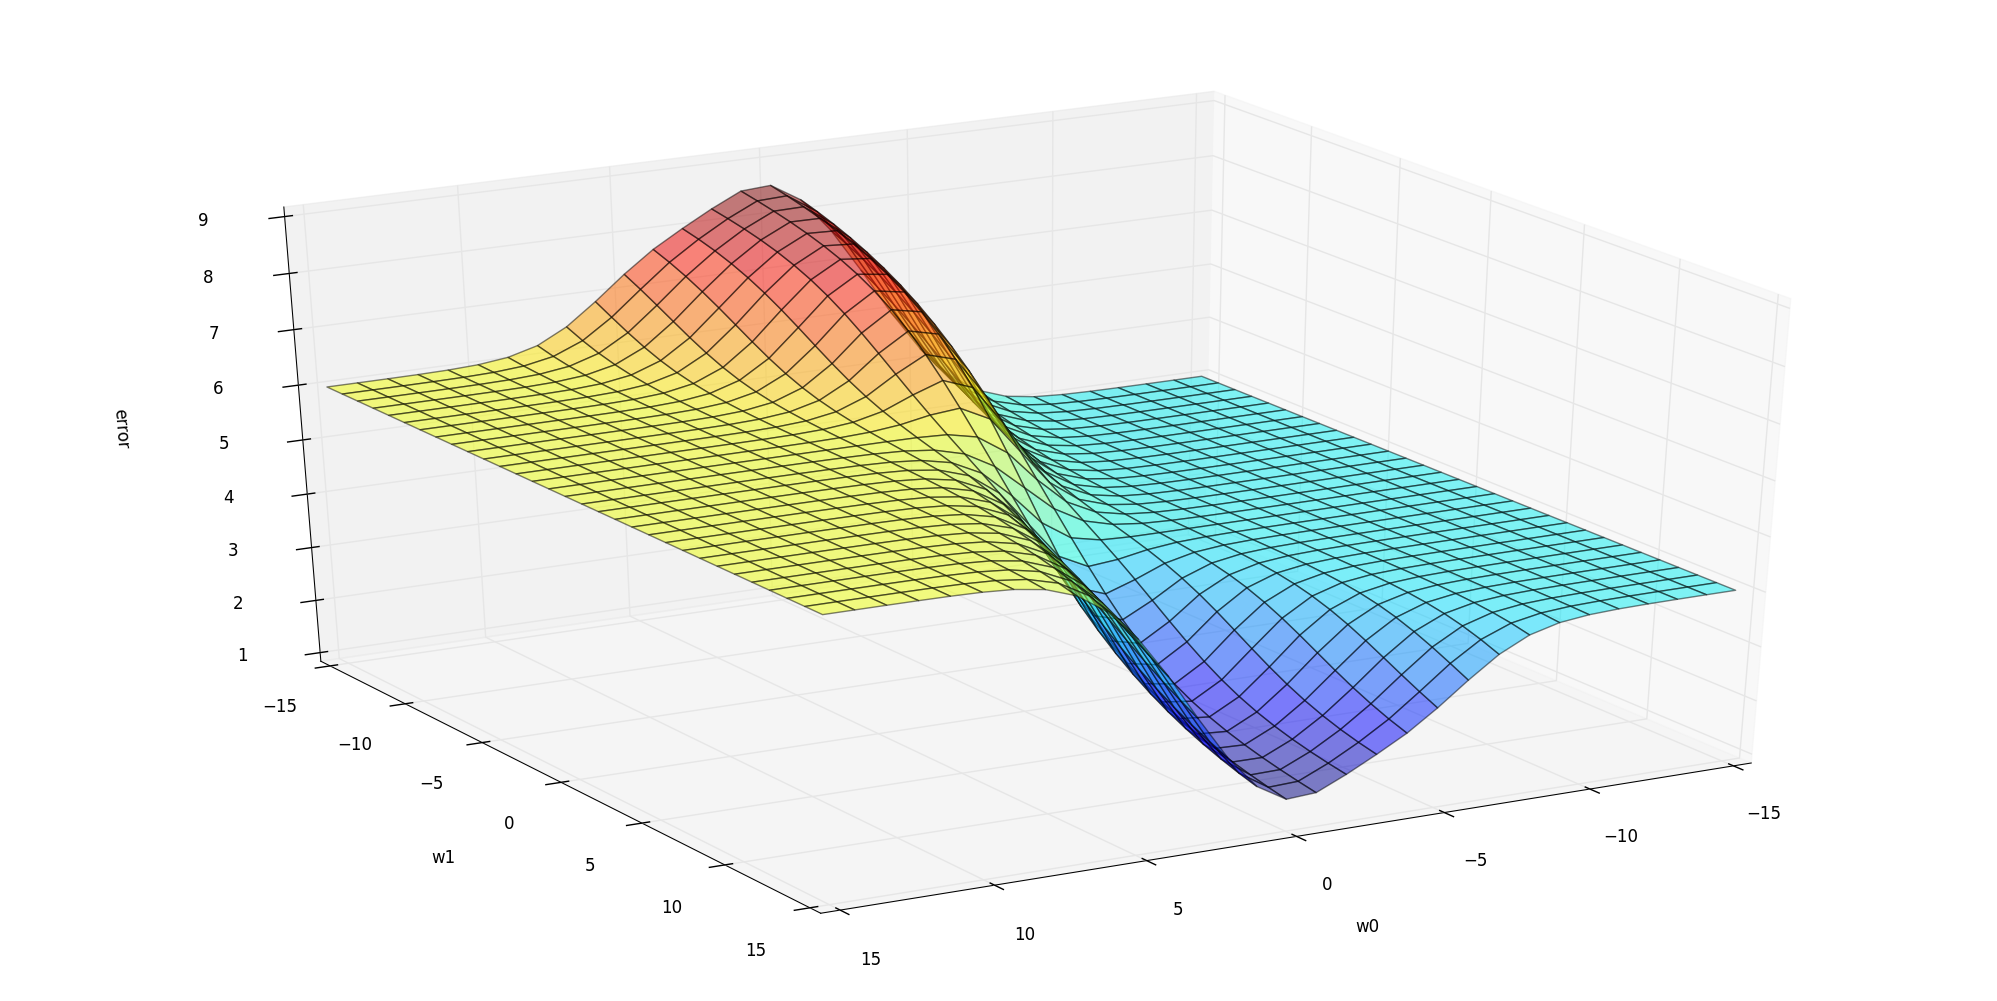
\includegraphics[scale=0.22]{./pictures/error_abs.png}
    \end{center}
  \end{frame}

  \begin{frame}
    \frametitle{The error function}
    \begin{center}
      \begin{equation*}
        \begin{split}
          e(w) & =
          \left \{
            \begin{array}{cl}
              -\log(h_w(x)) & $ if $ y = 1\\
              -\log(1 - h_w(x)) & $ if $ y = 0
            \end{array}
            \right.\\~\\
            & = -y \log(h_w(x)) - (1 - y) \log(1 - h_w(x))\\~\\
          \end{split}
        \end{equation*}
      \end{center}
    \end{frame}

    \begin{frame}
      \frametitle{The logistic function}
      \begin{center}
        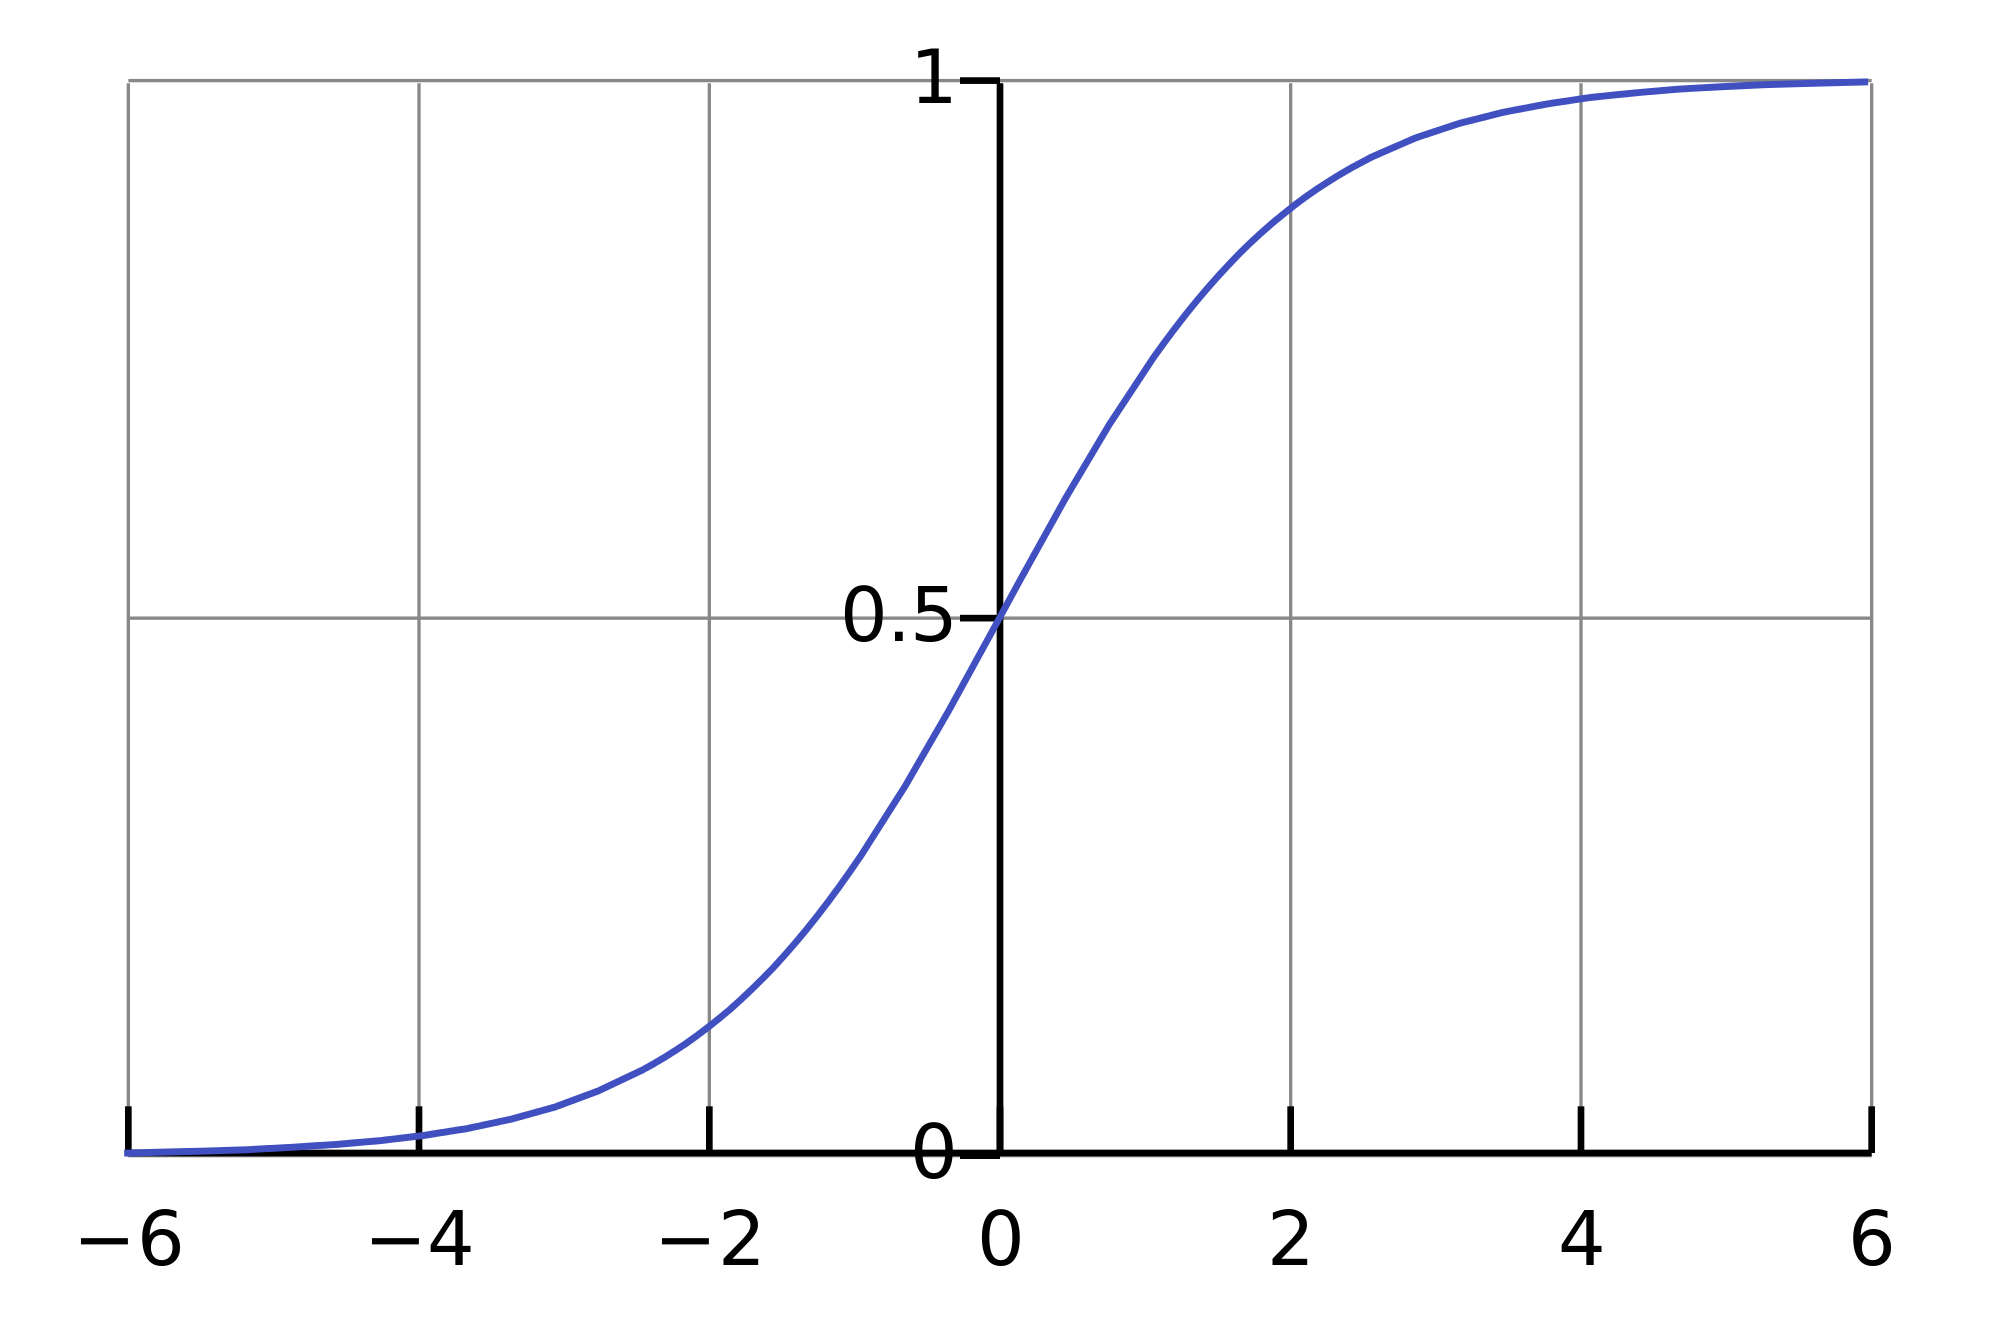
\includegraphics[scale=0.14]{./pictures/sigmoid.png}
      \end{center}
    \end{frame}

    \begin{frame}
      \frametitle{Error function}
      \begin{center}
        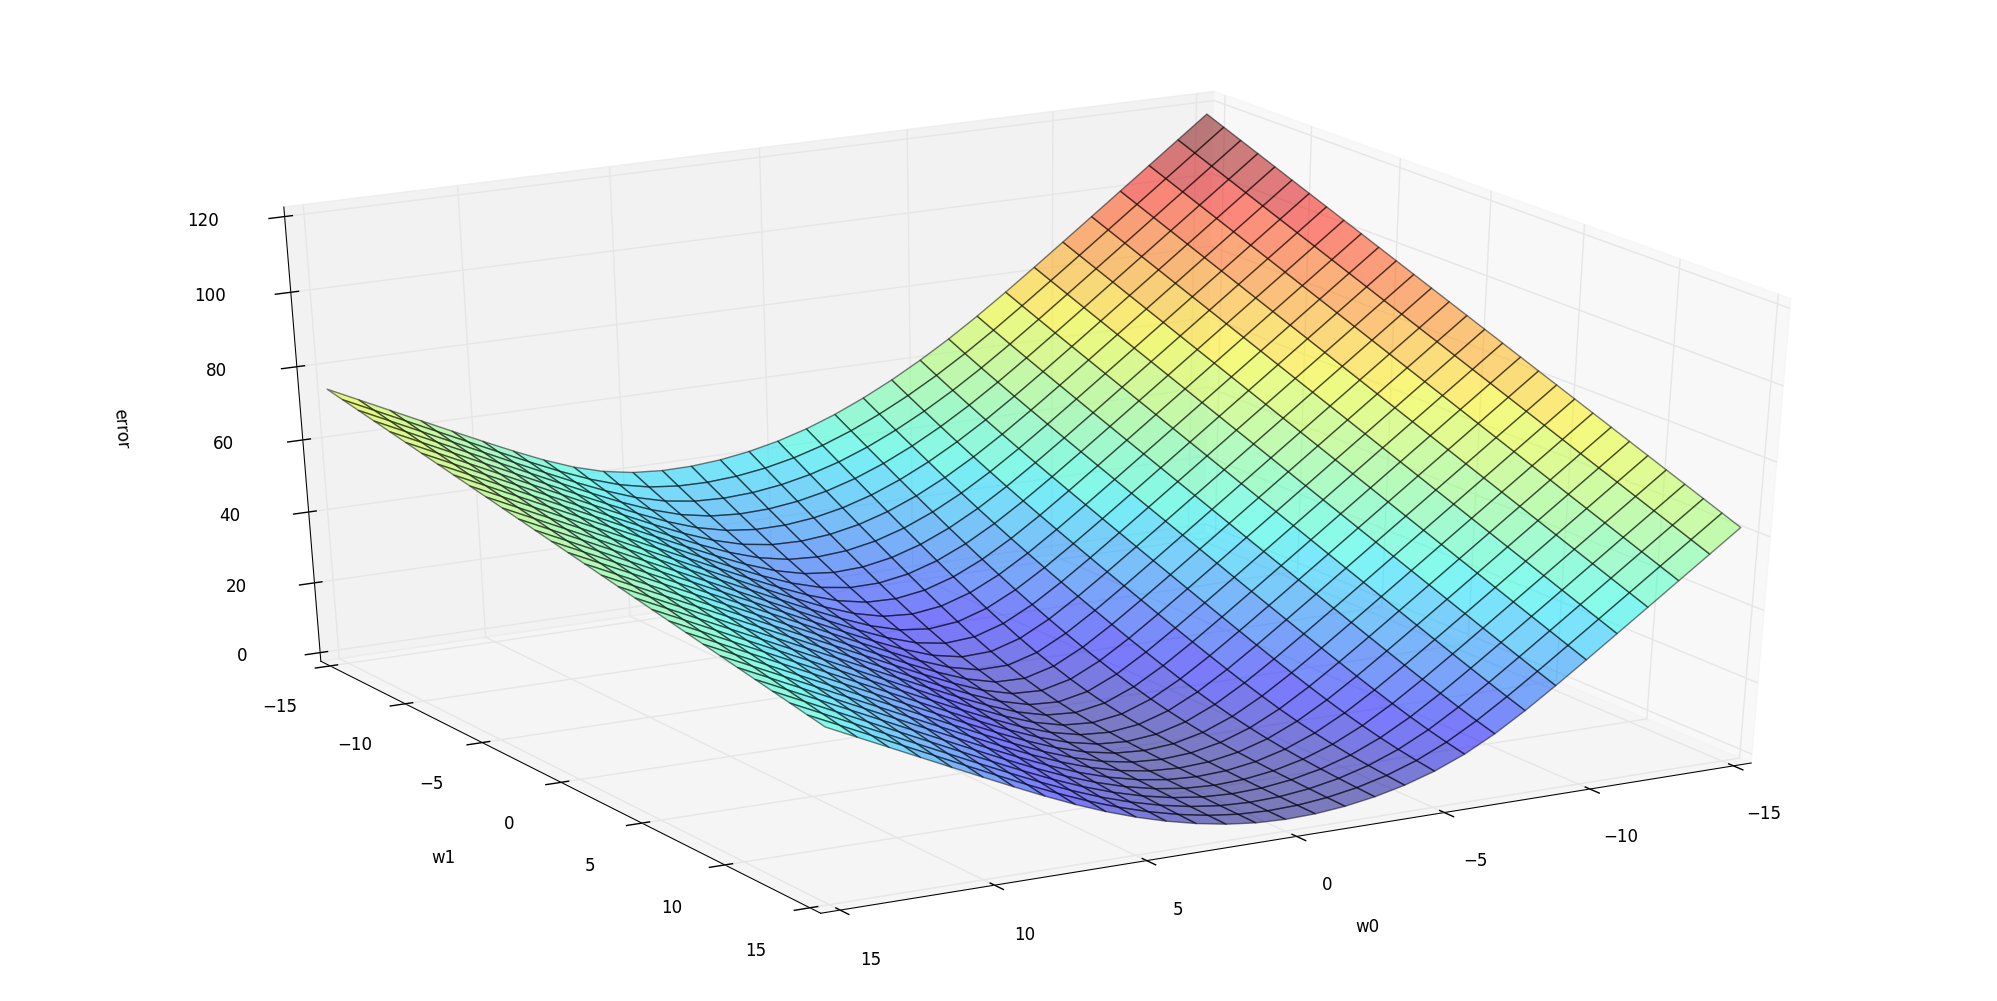
\includegraphics[scale=0.22]{./pictures/error_function.png}
      \end{center}
    \end{frame}

    \begin{frame}
      \begin{equation*}
        \begin{split}
          \frac{\partial e}{\partial w} & = \frac{\partial \displaystyle\sum_{i =
        1}^n{-y \log(h_w(x)) - (1 - y) \log(1 -
      h_w(x)})}{\partial w} \\~\\
      & = \displaystyle\sum_{i = 1}^n{\frac{\partial(-y \log(g(x \cdot
  w)) - (1 - y) \log(1 - g(x \cdot w)))}{\partial w}} \\
\end{split}
  \end{equation*}
\end{frame}

\begin{frame}
  \begin{equation*}
    E(w)
  \end{equation*}
\end{frame}

\begin{frame}[fragile]
  \begin{block}{Logistic function}
    \begin{lstlisting}
      def g(x):
      1 / (1 + exp(-x))
    \end{lstlisting}
  \end{block}
\end{frame}

\begin{frame}
  \frametitle{Gradient descent}
  \begin{center}
    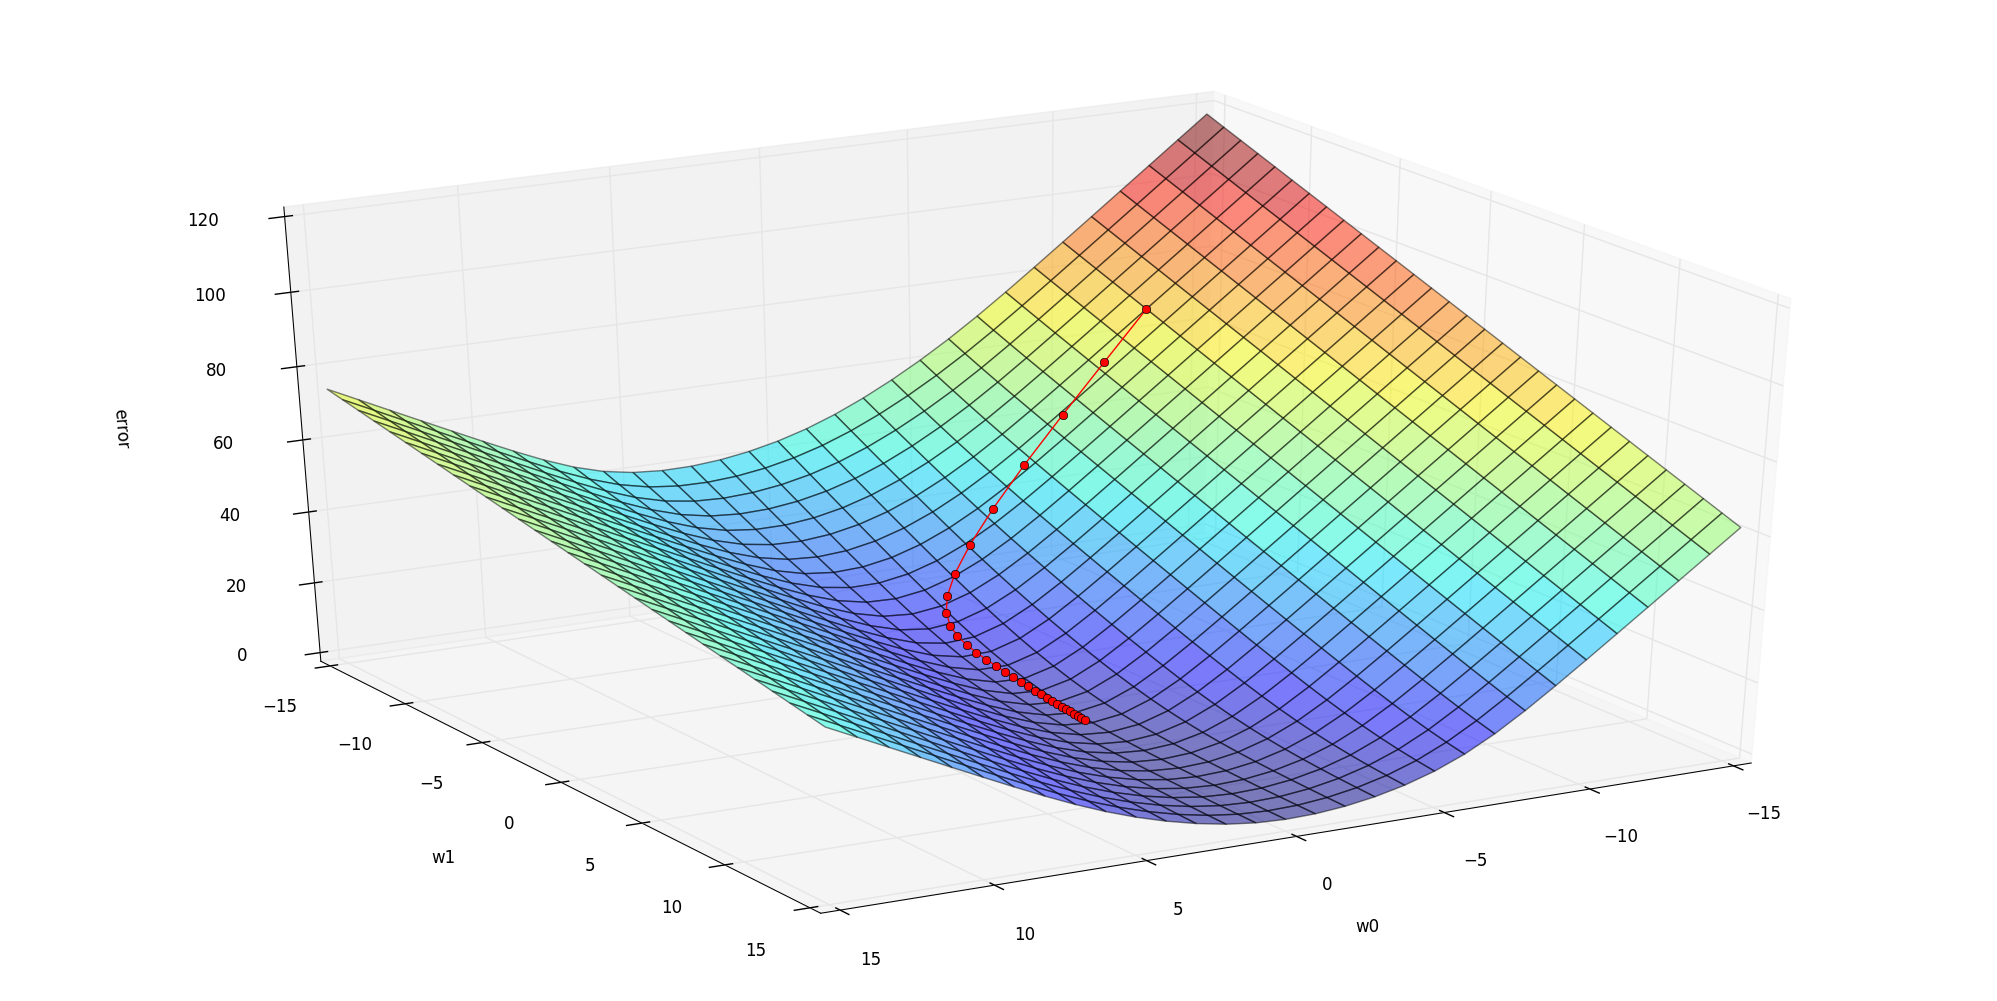
\includegraphics[scale=0.22]{./pictures/gradient_descent.png}
  \end{center}
\end{frame}

\begin{frame}
  \begin{tikzpicture}[shorten >=1pt,->,draw=black!50, node distance=2.5cm]
    \tikzstyle{every pin edge}=[<-,shorten <=1pt]
    \tikzstyle{neuron}=[circle,draw,minimum size=17pt,inner sep=0pt]

    \foreach \y in {1,2,3,4}
    \node[neuron, pin=left:$x\y$] (I-\y) at (0,-\y) {};

    \node[neuron,pin={[pin edge={->}]right:$y1$}, right of=I-3] (O-1) at
    (1.2,-2.5) {$g(\textbf{x} \cdot \textbf{w})$};

    \foreach \src in {1,2,3,4}
    \path (I-\src) edge (O-1);
  \end{tikzpicture}
\end{frame}

\begin{frame}
  \begin{center}
    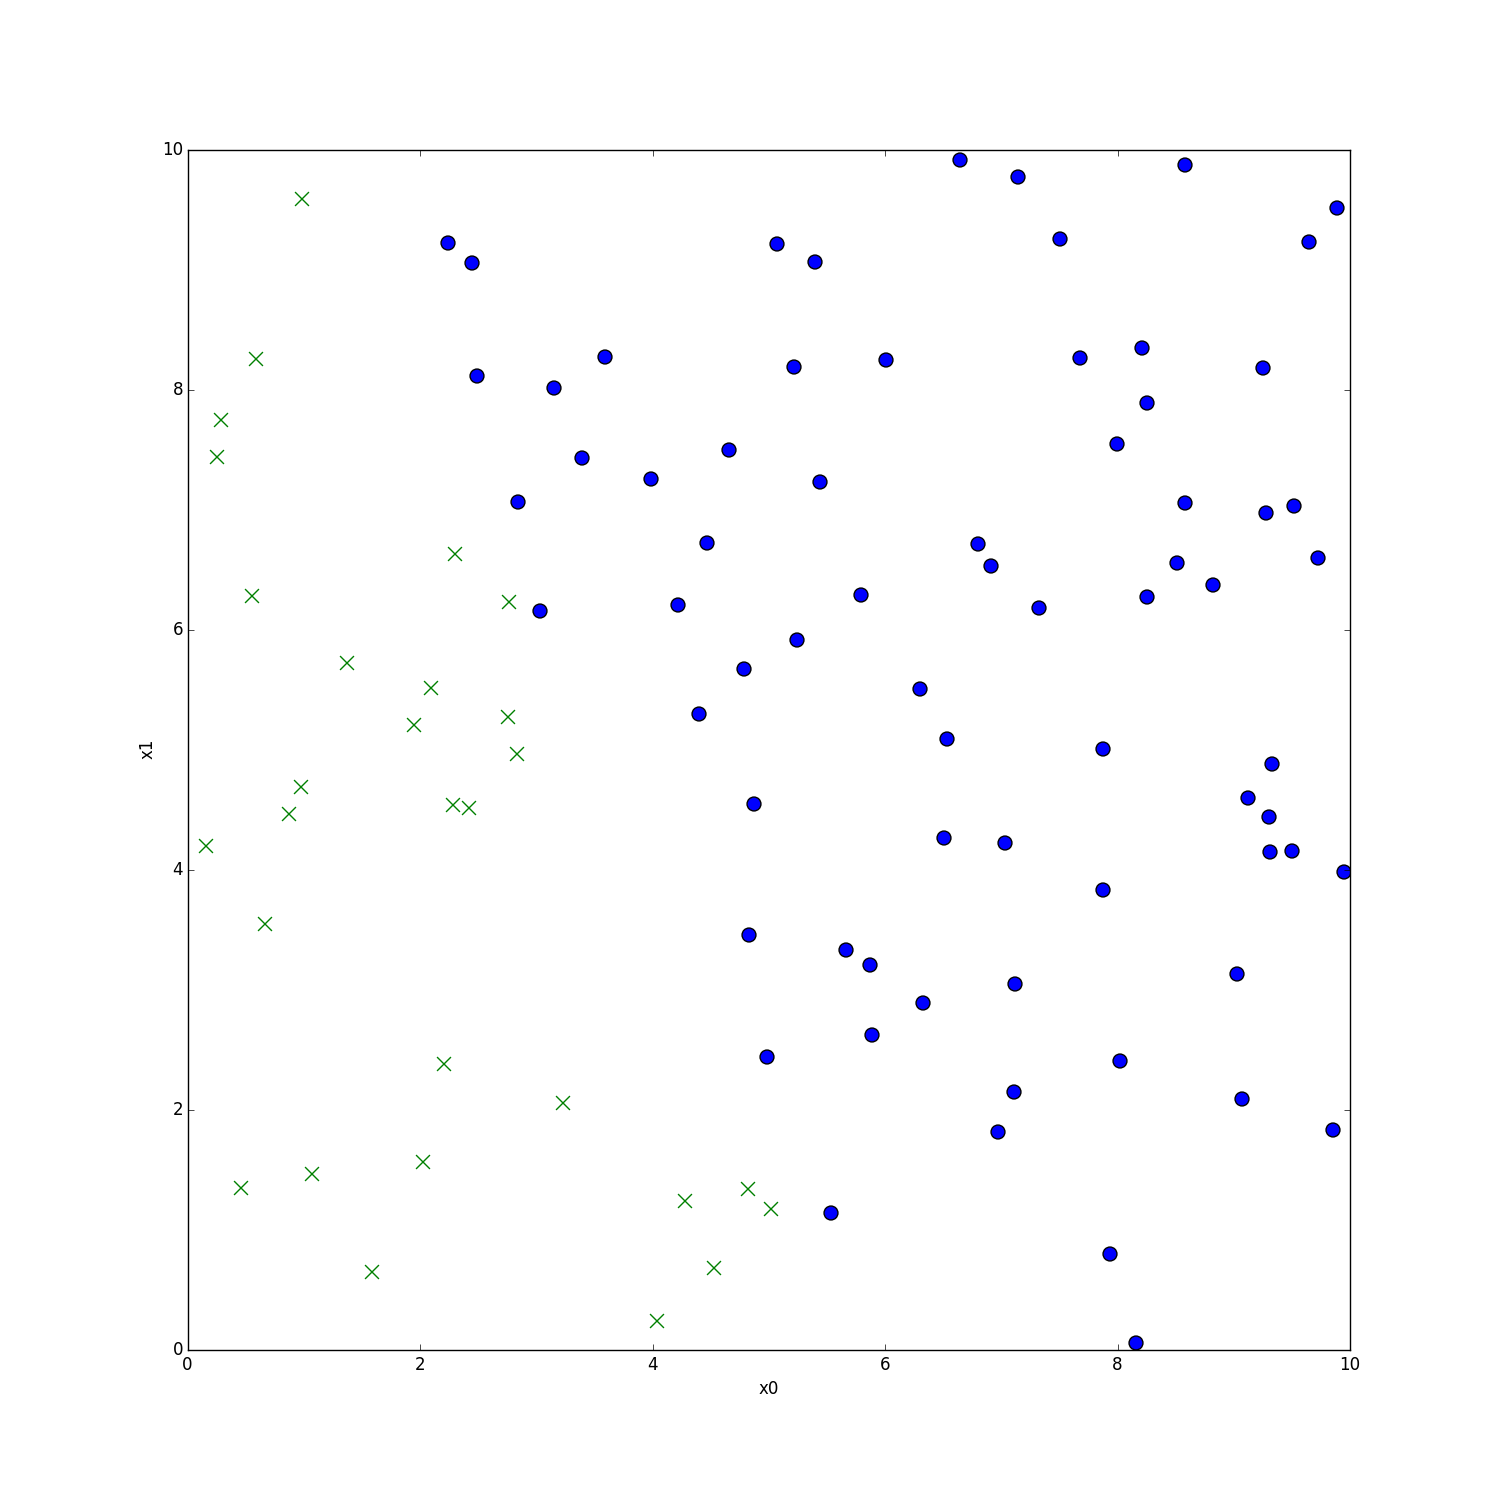
\includegraphics[scale=0.2]{./pictures/logreg_db000.png}
  \end{center}
\end{frame}

\begin{frame}
  \begin{center}
    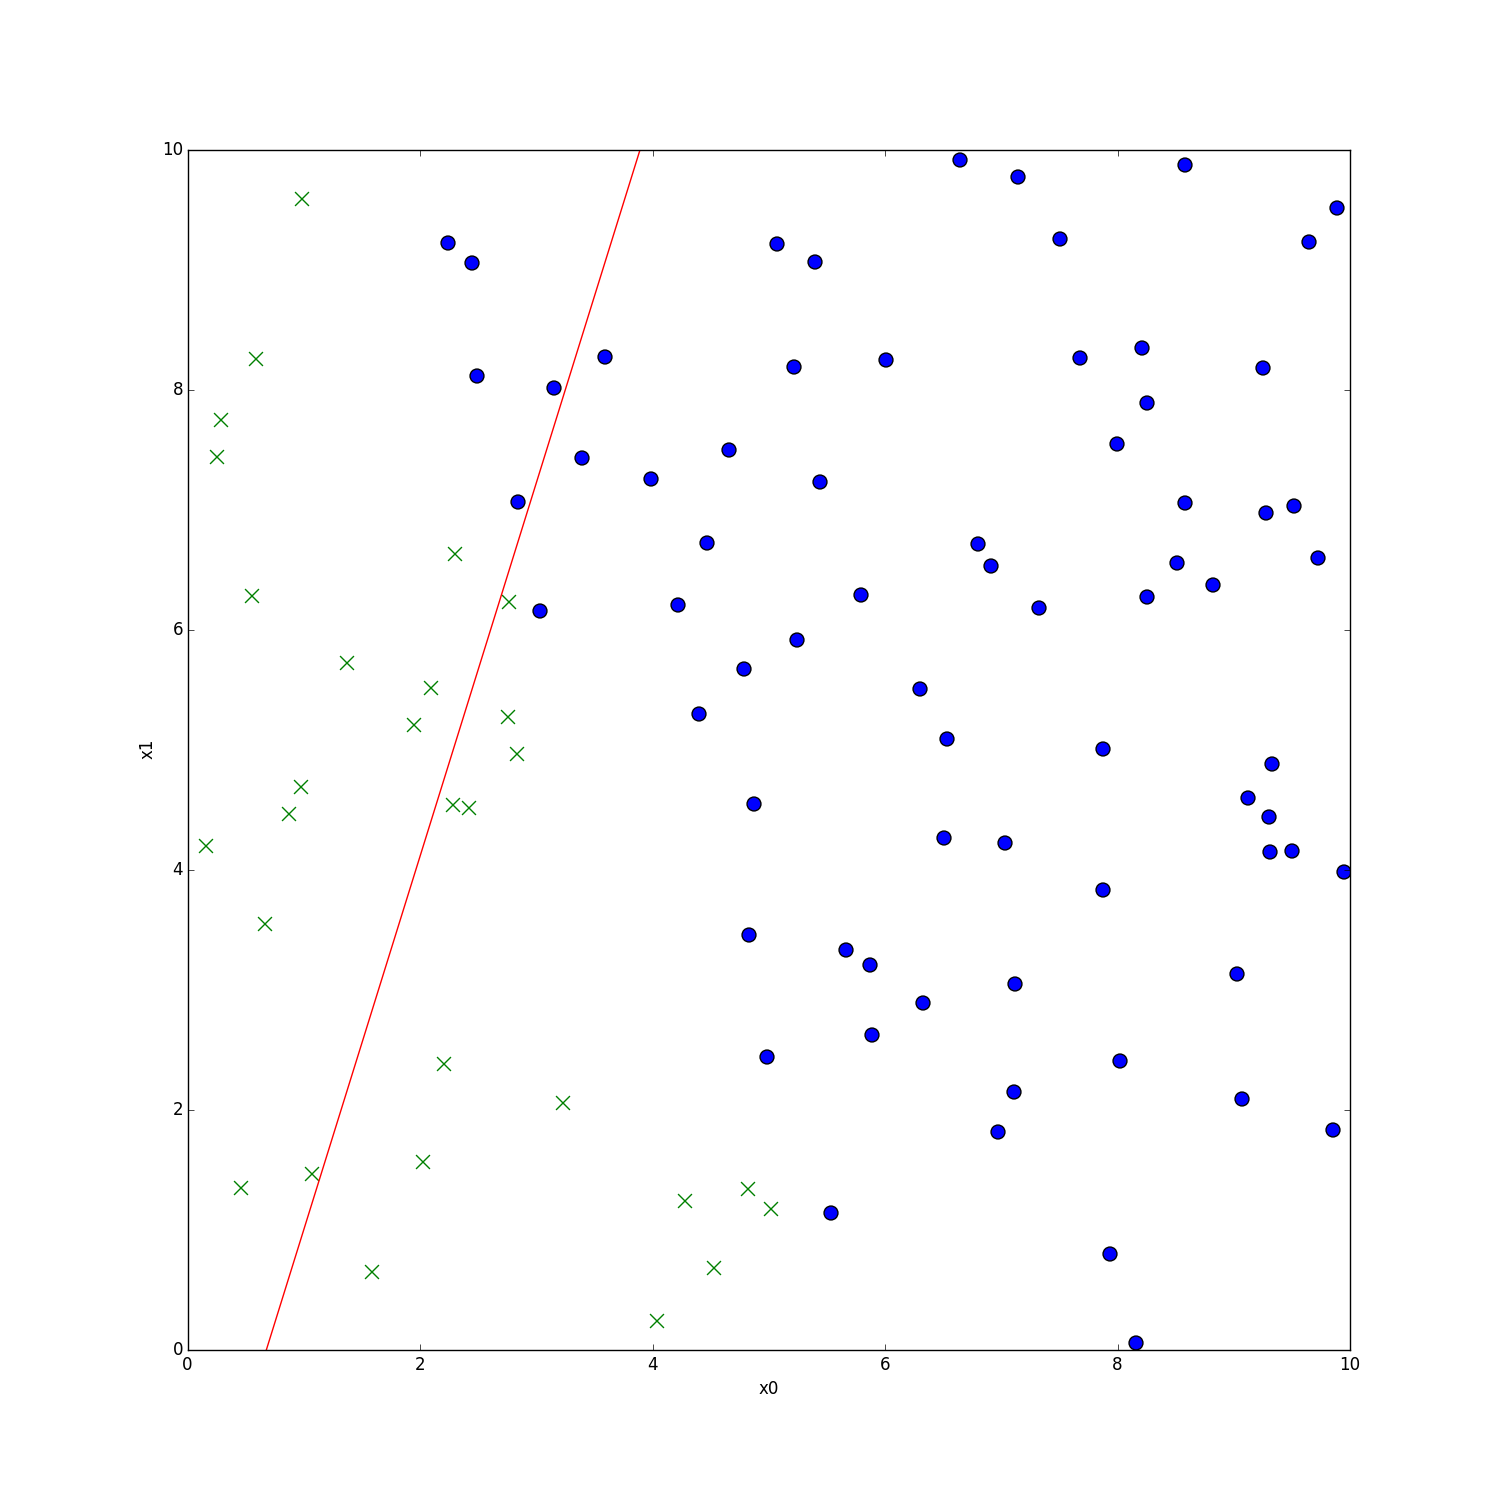
\includegraphics[scale=0.2]{./pictures/logreg_db001.png}
  \end{center}
\end{frame}

\begin{frame}
  \begin{center}
    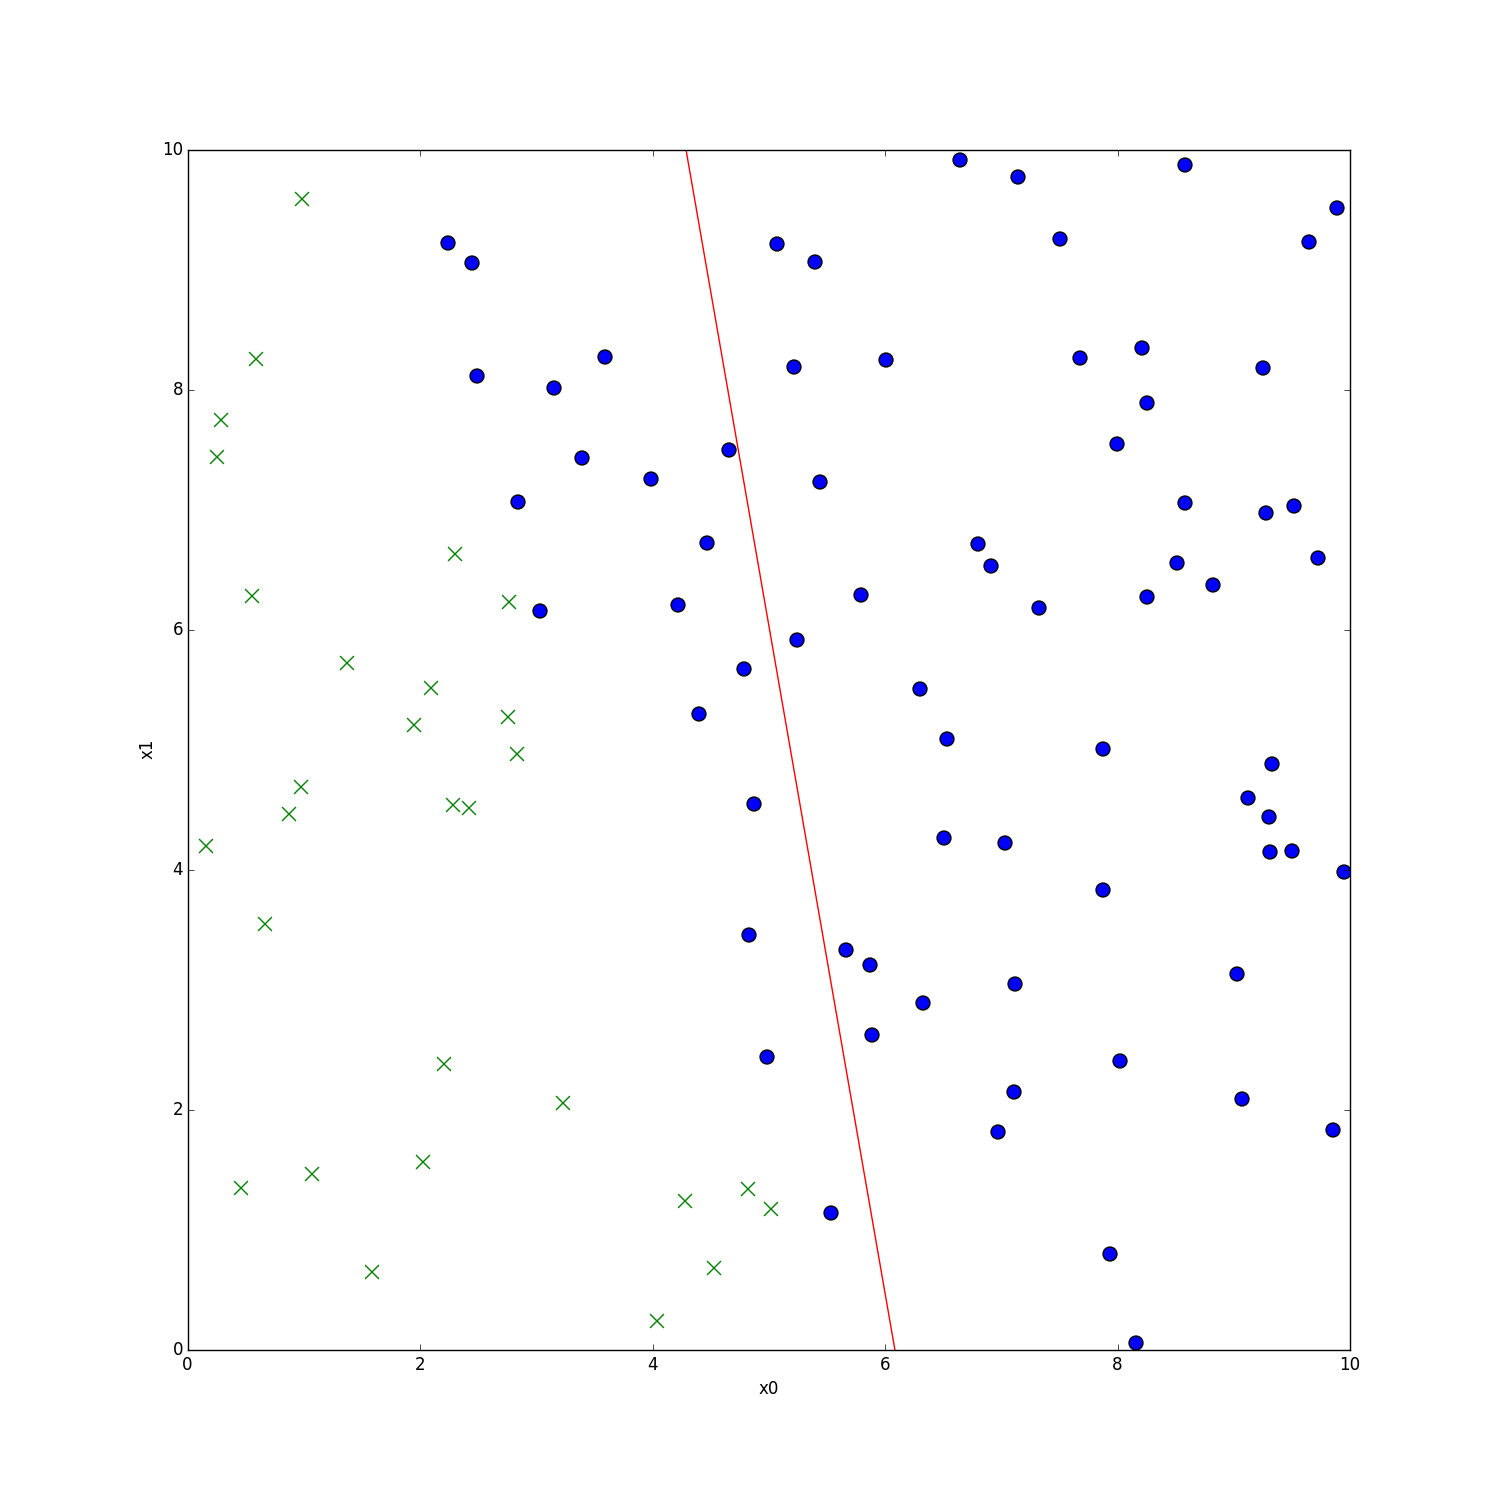
\includegraphics[scale=0.2]{./pictures/logreg_db012.png}
  \end{center}
\end{frame}

\begin{frame}
  \begin{center}
    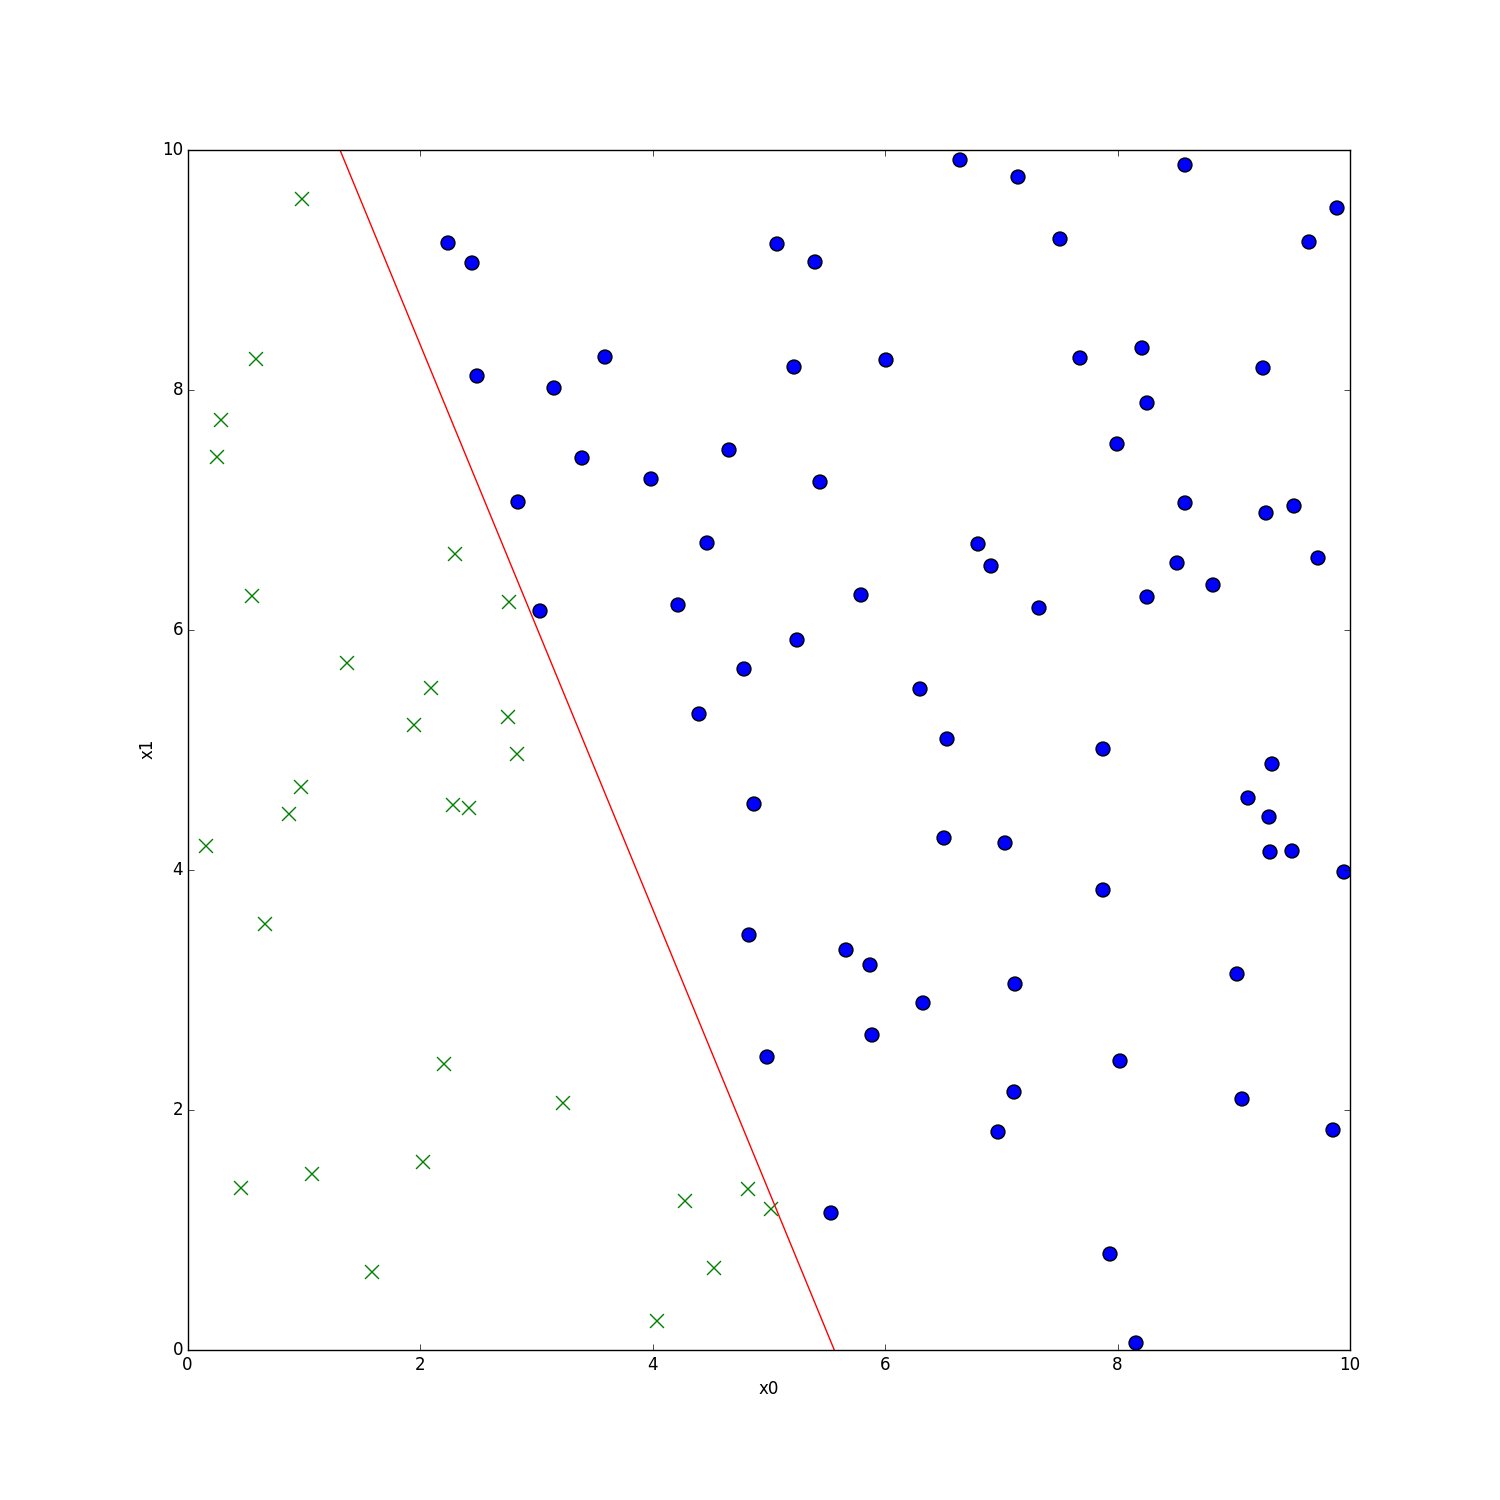
\includegraphics[scale=0.2]{./pictures/logreg_db078.png}
  \end{center}
\end{frame}

\begin{frame}
\begin{center}
  $
  \begin{array}{cc}
      &
      \left(
        \begin{matrix}
          \only<2>{w_0 \\}
          w_1 \\
          \vdots \\
          w_n
        \end{matrix}
      \right) \\
    &\\
    \left(
      \begin{matrix}
        \only<2>{1 &} x_1 & \ldots & x_{n}
      \end{matrix}
    \right) & {\left(\textbf{x} \cdot \textbf{w} \right)}
  \end{array}
  \hspace{2em}
  $
\only<1>{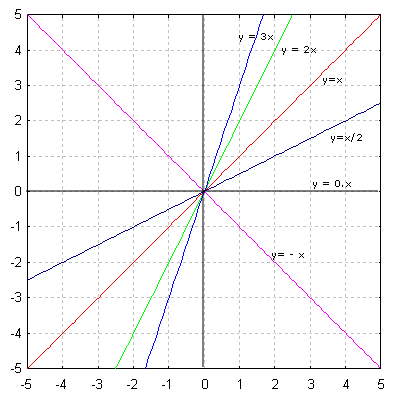
\includegraphics[scale=0.3]{./pictures/linear.png}}
\only<2>{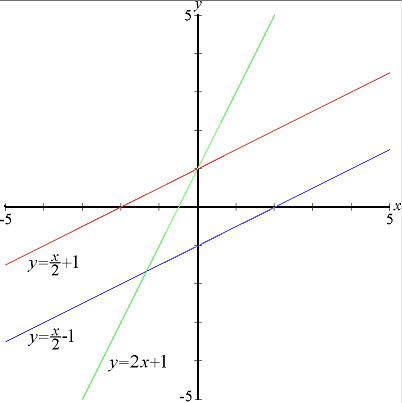
\includegraphics[scale=0.3]{./pictures/affine.png}}
\end{center}
\end{frame}


\section{Single layer perceptron}
\tableofcontents[sectionstyle=show/shaded]
\begin{frame}[fragile]
  \frametitle{Notation}
  $
  \begin{array}{cc}
      &
      \left(
        \begin{matrix}
          x_0 \\
          \vdots \\
          x_n
        \end{matrix}
      \right) \\
    &\\
    \left(
      \begin{matrix}
        w_{\only<2>{0}0} & \ldots & w_{\only<2>{0}n} \only<2>{\\
        \vdots & \ddots & \vdots \\
      w_{m0} & \ldots & w_{mn}}
      \end{matrix}
  \right) & {\left(
      \begin{matrix}
        net\only<2>{_0} \only<2>{\\
          \vdots \\
        net\only<2>{_m}}
      \end{matrix}
  \right)}
  \end{array}
  \qquad net = w^T \cdot x
  $
\end{frame}

\begin{frame}
  \begin{tikzpicture}[shorten >=1pt,->,draw=black!50, node distance=2.5cm]
    \tikzstyle{every pin edge}=[<-,shorten <=1pt]
    \tikzstyle{neuron}=[circle,draw,minimum size=17pt,inner sep=0pt]

    % input layer nodes
    \foreach \y in {1,...,4}
    \node[neuron, pin=left:$x\y$] (I-\y) at (0,-\y) {};

    % output layer node
    \path[yshift=-1.4cm]
    node[neuron,pin={[pin edge={->}]right:$o1 = P(x \in A)$}] (O-1) at (2.5,0) {};
    \path[yshift=-1.4cm]
    node[neuron,pin={[pin edge={->}]right:$o2 = P(x \in B)$}] (O-2) at (2.5,-1) {};
    \path[yshift=-1.4cm]
    node[neuron,pin={[pin edge={->}]right:$o3 = P(x \in C)$}] (O-3) at (2.5,-2) {};

    % Connect every node in the input layer with every node in the
    % output layer.
    \foreach \src in {1,...,4}
    \foreach \dst in {1,2,3}
    \ifthenelse{\equal{\dst}{1}}
    {\path[draw=red] (I-\src) edge (O-\dst)}
    {\path[draw=black!50] (I-\src) edge (O-\dst)};
  \end{tikzpicture}
\end{frame}

\begin{frame}[fragile]
  \hspace{2em}
  \begin{block}{Hypothesis}
    \begin{lstlisting}
def g(x):
    return 1 / (1 + exp(x))

def h(x, w):
    return transpose(w) * x
    \end{lstlisting}
  \end{block}
\end{frame}

\begin{frame}
\end{frame}

\begin{frame}[fragile]
  \begin{block}{Hypothesis function}
      \begin{lstlisting}
def gradient(x, y, w):
    d = h(x, w) - y
    return x * transpose(d)
      \end{lstlisting}
  \end{block}
\end{frame}

\begin{frame}
  $
  \begin{array}{cc}
    &
    \left(
      \begin{matrix}
        d\only<2>{_1& \ldots & d_{m}} \\
      \end{matrix}
    \right) \\
    &\\
    \left(
      \begin{matrix}
        x_{1} \\
        \vdots \\
        x_{n}
      \end{matrix}
    \right) & \left(
      \only<1>{\begin{matrix}
        x_0 d \\
        \vdots \\
        x_n d
      \end{matrix}}
      \only<2>{\begin{matrix}
        x_0 d_0 & \ldots & x_0 d_m \\
        \vdots & \ddots & \vdots \\
        x_n d_0 & \ldots & x_n d_m
      \end{matrix}}
    \right)
  \end{array}
  \qquad \frac{\partial E}{\partial w_{i\only<2>{j}}} = x_i d\only<2>{_j}
  $
\end{frame}


\section{Multilayer perceptron}
\tableofcontents[sectionstyle=show/shaded]
\begin{frame}
  \begin{center}
    {\Large Why do we need multiple layers?}
  \end{center}
\end{frame}

\begin{frame}
  \begin{center}
    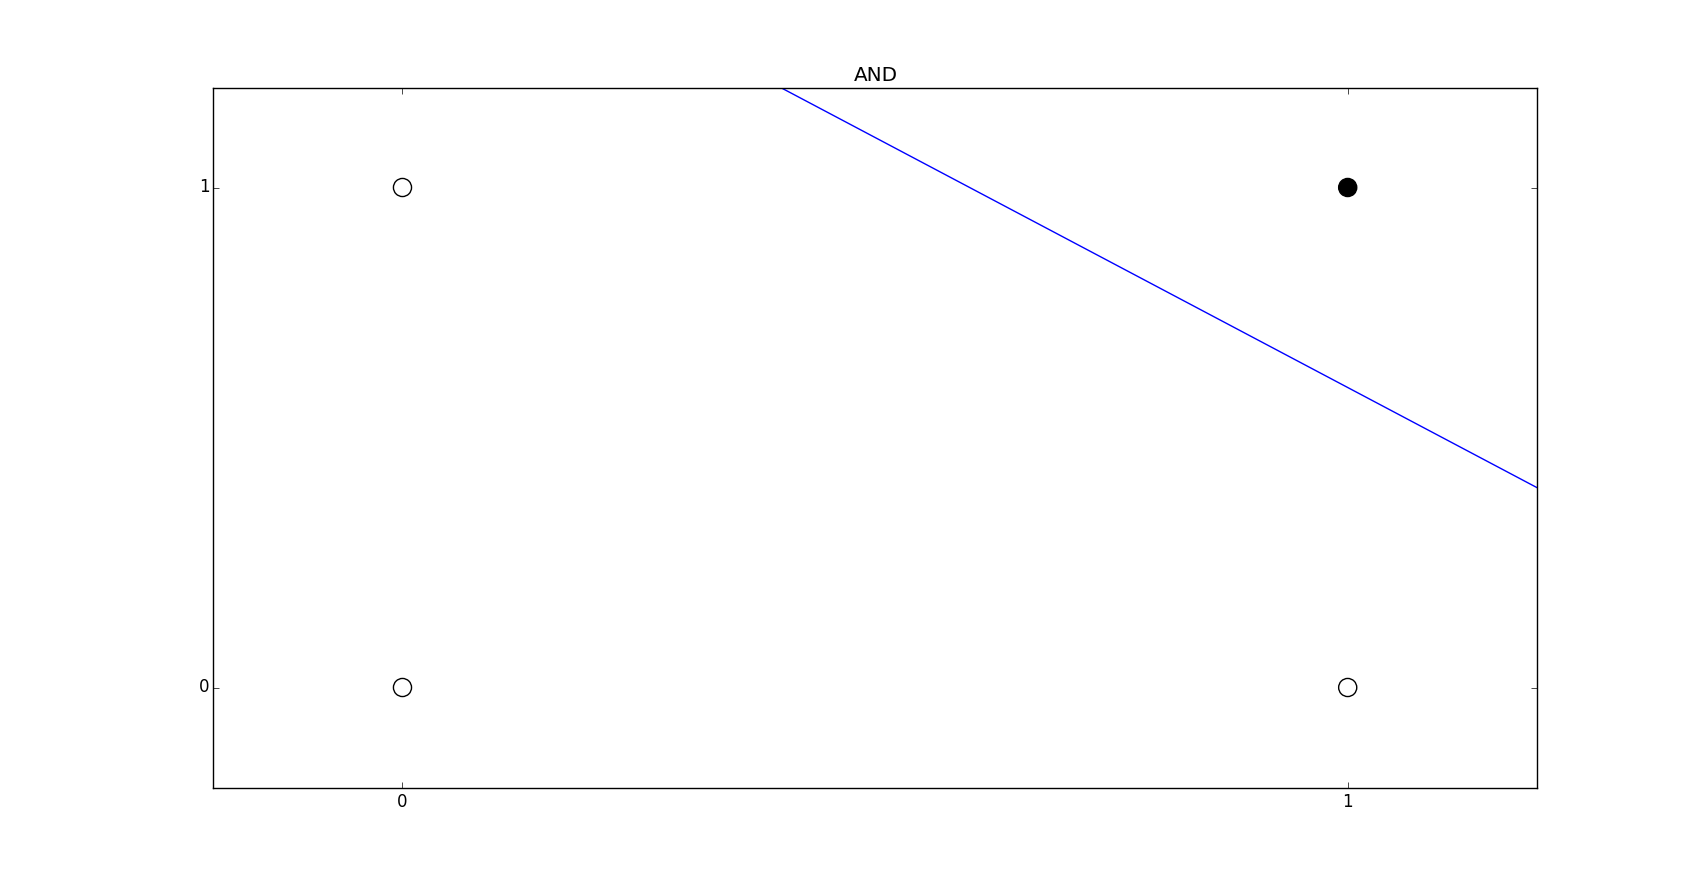
\includegraphics[scale=0.25]{pictures/and.png}
  \end{center}
\end{frame}

\begin{frame}
  \begin{center}
    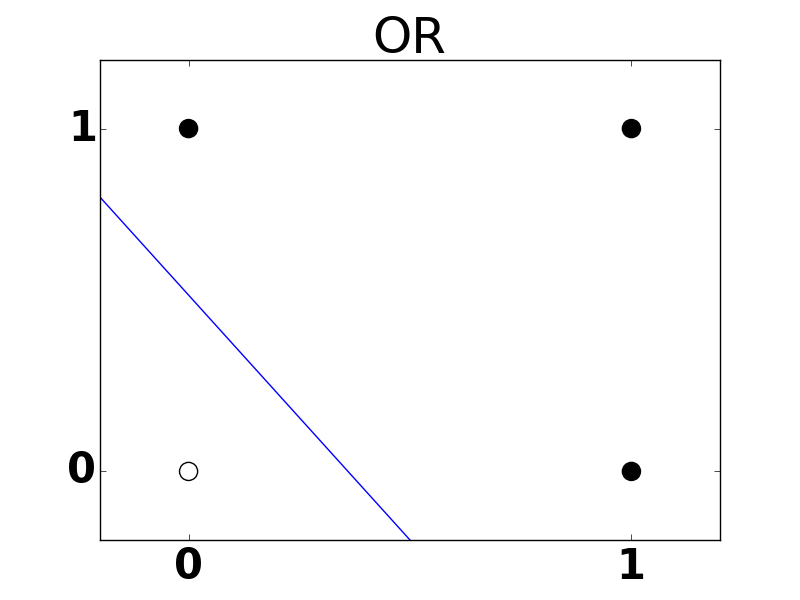
\includegraphics[scale=0.25]{pictures/or.png}
  \end{center}
\end{frame}

\begin{frame}
  \begin{center}
    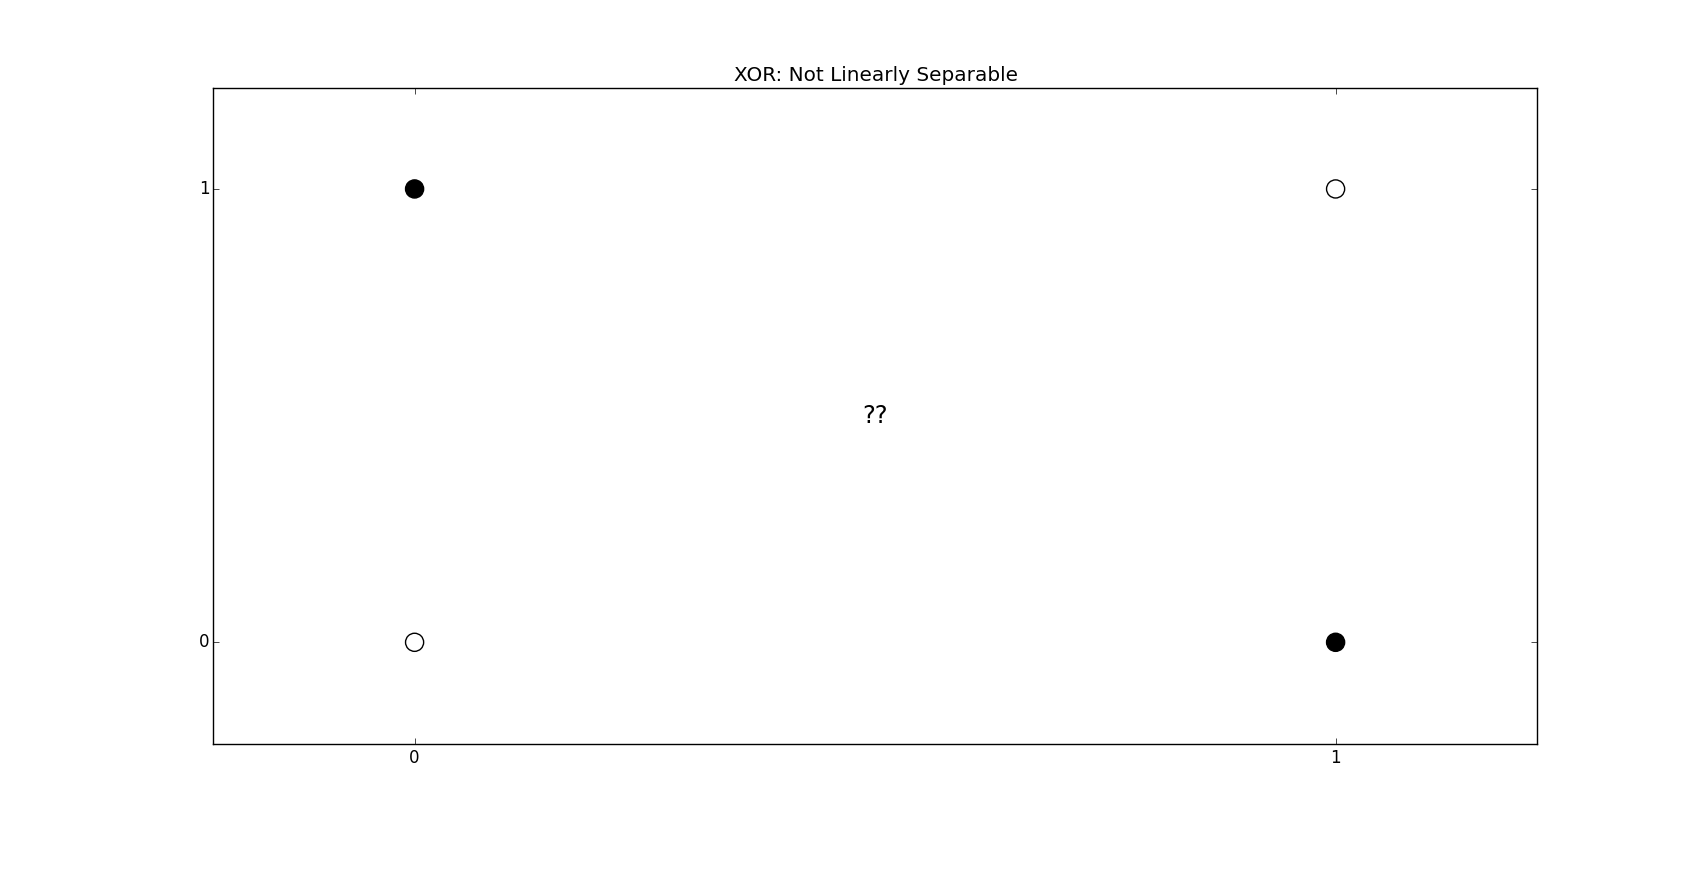
\includegraphics[scale=0.25]{pictures/xor.png}
  \end{center}
\end{frame}

\begin{frame}[fragile]
  \begin{block}{Forward propagation}
    \begin{lstlisting}
def add_bias(o):
    return insert(o, 0, 1, axis=0)
|\pause|
def h(x, w):
    out = [x]|\pause|
    for l in range(len(w)):|\pause|
        x = add_bias(out[l])|\pause|
        o = g(transpose(w[l]) * x)|\pause|
        out.append(o)|\pause|
    return out
  \end{lstlisting}
  \end{block}
\end{frame}
% Linearly separable data vs non-linearly separable data.


\begin{frame}
  \begin{center}
  \begin{tikzpicture}[shorten >=1pt,->,draw=black!50, node distance=2.5cm]
    \tikzstyle{every pin edge}=[<-,shorten <=1pt]
    \tikzstyle{neuron}=[circle,draw,minimum size=17pt,inner sep=0pt]

    % input layer nodes
    \foreach \y in {1,...,4}
    \node[neuron, pin=left:$x\y$] (I-\y) at (0,-\y) {};

    % hidden layer nodes
    \foreach \y in {1,...,5}
    \path[yshift=0.5cm]
    node[neuron] (H-\y) at (2.5,-\y) {};

    % output layer node
    \foreach \y in {1,2}
    \path[yshift=-1cm]
    node[neuron,pin={[pin edge={->}]right:$o\y$}] (O-\y) at (4.5,-\y) {};

    % Connect every node in the input layer with every node in the
    % hidden layer.
    \foreach \src in {1,...,4}
    \foreach \dst in {1,...,5}
    \path[draw=black,thick] (I-\src) edge (H-\dst);

    % Connect every node in the hidden layer with the output layer
    \foreach \src in {1,...,5}
    \foreach \dst in {1,2}
    \path (H-\src) edge (O-\dst);
  \end{tikzpicture}
  \end{center}
\end{frame}

\begin{frame}
  \begin{center}
  \begin{tikzpicture}[shorten >=1pt,->,draw=black!50, node distance=2.5cm]
    \tikzstyle{every pin edge}=[<-,shorten <=1pt]
    \tikzstyle{neuron}=[circle,draw,minimum size=17pt,inner sep=0pt]

    % input layer nodes
    \foreach \y in {1,...,4}
    \node[neuron, pin=left:$x\y$] (I-\y) at (0,-\y) {};

    % hidden layer nodes
    \foreach \y in {1,...,5}
    \path[yshift=0.5cm]
    node[neuron] (H-\y) at (2.5,-\y) {};

    % output layer node
    \foreach \y in {1,2}
    \path[yshift=-1cm]
    node[neuron,pin={[pin edge={->}]right:$o\y$}] (O-\y) at (4.5,-\y) {};

    % Connect every node in the input layer with every node in the
    % hidden layer.
    \foreach \src in {1,...,4}
    \foreach \dst in {1,...,5}
    \path (I-\src) edge (H-\dst);

    % Connect every node in the hidden layer with the output layer
    \foreach \src in {1,...,5}
    \foreach \dst in {1,2}
    \path[draw=black,thick] (H-\src) edge (O-\dst);
  \end{tikzpicture}
  \end{center}
\end{frame}

% if input is (x1, x2), add x1^2, x2^2 and x1x2 as inputs

\begin{frame}
  \begin{tikzpicture}[shorten >=1pt,->,draw=black!50, node distance=2.5cm]
    \tikzstyle{every pin edge}=[<-,shorten <=1pt]
    \tikzstyle{neuron}=[circle,draw,minimum size=17pt,inner sep=0pt]

    % input layer nodes
    \foreach \y in {1,...,2}
    \node[neuron, pin=left:$x\y$] (I-\y) at (0,-\y) {};

    % hidden layer nodes
    \foreach \y in {1,...,2}
    \path[yshift=0cm]
    node[neuron] (H-\y) at (2.5,-\y) {};

    % output layer node
    \foreach \y in {1}
    \path[yshift=-0.5cm]
    node[neuron,pin={[pin edge={->}]right:$y\y$}, right of=H-2] (O-\y) at (2.7,-\y) {};

    % Connect every node in the input layer with every node in the
    % hidden layer.
    \foreach \src in {1,...,2}
    \foreach \dst in {1,...,2}
    \path (I-\src) edge (H-\dst);

    % Connect every node in the hidden layer with the output layer
    \foreach \src in {1,...,2}
    \foreach \dst in {1}
    \path (H-\src) edge (O-\dst);
  \end{tikzpicture}
\end{frame}


\section{Backpropagation algorithm}
\tableofcontents[sectionstyle=show/shaded]
\begin{frame}
  \begin{tikzpicture}[shorten >=1pt,->,draw=black!50, node distance=2.5cm]
    \tikzstyle{every pin edge}=[<-,shorten <=1pt]
    \tikzstyle{neuron}=[circle,draw,minimum size=17pt,inner sep=0pt]

    % input layer nodes
    \foreach \y in {1,...,4}
    \node[neuron, pin=left:$x\y$] (I-\y) at (0,-\y) {};

    % hidden layer nodes
    \foreach \y in {1,...,5}
    \path[yshift=0.5cm]
    node[neuron] (H-\y) at (2.5,-\y) {};

    % output layer node
    \foreach \y in {1,2}
    \path[yshift=-1cm]
    node[neuron,pin={[pin edge={->}]right:$o\y$}] (O-\y) at (4.5,-\y) {};

    % Connect every node in the input layer with every node in the
    % hidden layer.
    \foreach \src in {1,...,4}
    \foreach \dst in {1,...,5}
    \path (I-\src) edge (H-\dst);

    % Connect every node in the hidden layer with the output layer
    \foreach \src in {1,...,5}
    \foreach \dst in {1,2}
    \path[draw=black,thick] (H-\src) edge (O-\dst);
  \end{tikzpicture}
\end{frame}

\begin{frame}
  \begin{tikzpicture}[shorten >=1pt,->,draw=black!50, node distance=2.5cm]
    \tikzstyle{every pin edge}=[<-,shorten <=1pt]
    \tikzstyle{neuron}=[circle,draw,minimum size=17pt,inner sep=0pt]

    % input layer nodes
    \foreach \y in {1,...,4}
    \node[neuron, pin=left:$x\y$] (I-\y) at (0,-\y) {};

    % hidden layer nodes
    \foreach \y in {1,...,5}
    \path[yshift=0.5cm]
    node[neuron] (H-\y) at (2.5,-\y) {};

    % output layer node
    \foreach \y in {1,2}
    \path[yshift=-1cm]
    node[neuron,pin={[pin edge={->}]right:$o\y$}] (O-\y) at (4.5,-\y) {};

    % Connect every node in the input layer with every node in the
    % hidden layer.
    \foreach \src in {1,...,4}
    \foreach \dst in {1,...,5}
    \path[draw=black,thick] (I-\src) edge (H-\dst);

    % Connect every node in the hidden layer with the output layer
    \foreach \src in {1,...,5}
    \foreach \dst in {1,2}
    \path (H-\src) edge (O-\dst);
  \end{tikzpicture}
\end{frame}

\begin{frame}
  \begin{equation*}
    \begin{split}
      \frac{\partial E}{\partial w_{ij}} & = \frac{\partial E}{\partial o_j}
      \cdot \frac{\partial o_j}{\partial net_j} \cdot \frac{\partial
      net_j}{\partial w_{ij}}
    \end{split}
  \end{equation*}

  \begin{tikzpicture}[shorten >=1pt,->,draw=black!50, node distance=2.5cm]
    \tikzstyle{every pin edge}=[<-,shorten <=1pt]
    \tikzstyle{neuron}=[circle,draw,minimum size=17pt,inner sep=0pt]

    % input layer nodes
    \foreach \y in {1,...,4}
    \node[neuron, pin=left:$x\y$] (I-\y) at (0,-\y) {};

    % hidden layer nodes
    \foreach \y in {1,...,5}
    \path[yshift=0.5cm]
    node[neuron] (H-\y) at (2.5,-\y) {};

    % output layer node
    \path[yshift=-2cm]
    node[neuron,pin={[pin edge={->,draw=black,thick}]right:$o1$},
    draw=black,thick] (O-1) at (4.5,0) {$net_1$}
    node[neuron,pin={[pin edge={->}]right:$o2$}] (O-2) at (4.5,-1) {};

    % Connect every node in the input layer with every node in the
    % hidden layer.
    \foreach \src in {1,...,4}
    \foreach \dst in {1,...,5}
    \path (I-\src) edge (H-\dst);

    % Connect every node in the hidden layer with the output layer
    \foreach \src in {1,...,5}
    \foreach \dst in {1,2}
    \ifthenelse{\equal{\src}{4}\and\equal{\dst}{1}}
    {\path[draw=black,thick] (H-\src) edge node[below,right] {$w_{41}$} (O-\dst) {}}
    {\path (H-\src) edge (O-\dst)};
  \end{tikzpicture}
\end{frame}

\begin{frame}
  \begin{equation*}
    \begin{split}
      \frac{\partial net_j}{\partial w_{ij}} & = \frac{\partial}{\partial
    w_{ij}}(w_{0j} x_0 + \ldots + w_{ij} x_i + \ldots + w_{nj} x_n) \\
    & = x_i \\
    \frac{\partial o_j}{\partial net_j} & = \frac{\partial}{\partial
  w_{ij}}g(net_j) \\
  & = g(net_j) (1 - g(net_j)) \\
  & = oj(1 - oj) \\
      \frac{\partial E}{\partial o_j} & = \frac{\partial}{\partial o_j}(-y_j
      \log(o_j) - (1 - y_j) \log(1 - o_j))\\
      & = -y_j \frac{1}{o_j} - (1 - y_j) \frac{-1}{1 - o_j} \\
    \end{split}
  \end{equation*}
\end{frame}

\begin{frame}
  \begin{equation*}
    \begin{split}
      \frac{\partial E}{\partial w_{ij}} & = \frac{\partial E}{\partial o_j}
    \cdot \frac{\partial o_j}{\partial net_j} \cdot \frac{\partial
    net_j}{\partial w_{ij}} \\
    & = (-y_j \frac{1}{o_j} - (1 - y_j) \frac{-1}{1 - o_j}) oj(1 - o_j) x_i \\
    & = (-y_j \frac{1}{o_j} + \frac{1}{1 - o_j} - \frac{y_j}{1 - o_j}) o_j(1 - oj) x_i \\
    & = (-y_j \frac{1 - o_j}{o_j} + 1 - y_j) o_j x_i \\
    & = \underbrace{(o_j - y_j)}_{\delta_j} x_i \\
  \end{split}
\end{equation*}
\end{frame}

% \begin{frame}[fragile]
%   \begin{block}{Backpropagation}
%     \begin{lstlisting}
% def gradient(out, y, w):|\pause|
%     L = len(out) - 1|\pause|
%     x = add_bias(out[L - 1])|\pause|
%     d = out[L] - y|\pause|
%     grad = [x * transpose(d)]|\pause|
%     ...
%     \end{lstlisting}
%   \end{block}
% \end{frame}

\begin{frame}
  \begin{equation*}
    \begin{split}
      \frac{\partial E}{\partial w_{ij}} & = \frac{\partial E}{\partial o_j}
      \only<1>{\cdot \frac{\partial o_j}{\partial net_j} \cdot \frac{\partial
      net_j}{\partial w_{ij}}} \only<2>{o_j (1 - o_j) x_i}
    \end{split}
  \end{equation*}
  \begin{tikzpicture}[shorten >=1pt,->,draw=black!50, node distance=2.5cm]
    \tikzstyle{every pin edge}=[<-,shorten <=1pt]
    \tikzstyle{neuron}=[circle,draw,minimum size=17pt,inner sep=0pt]

    % input layer nodes
    \foreach \y in {1,...,4}
    \node[neuron, pin=left:$x\y$] (I-\y) at (0,-\y) {};

    % hidden layer nodes
    \path[yshift=0.5cm]
    node[neuron] (H-1) at (2.5,-1) {}
    node[neuron] (H-2) at (2.5,-2) {}
    node[neuron] (H-3) at (2.5,-3) {}
    node[neuron,draw=black,thick,label=right:{$o4$}] (H-4) at (2.5,-4) {$net_4$}
    node[neuron] (H-5) at (2.5,-5) {};

    % output layer node
    \path[yshift=-2cm]
    node[neuron,pin={[pin edge={->}]right:$o1$}] (O-1) at (4.5,0) {}
    node[neuron,pin={[pin edge={->}]right:$o2$}] (O-2) at (4.5,-1) {};

    % Connect every node in the input layer with every node in the
    % hidden layer.
    \foreach \src in {1,...,4}
    \foreach \dst in {1,...,5}
    \ifthenelse{\equal{\src}{2}\and\equal{\dst}{4}}
    {\path[draw=black,thick] (I-\src) edge node[above] {$w_{24}$} (H-\dst)}
    {\path (I-\src) edge (H-\dst)};

    % Connect every node in the hidden layer with the output layer
    \foreach \src in {1,...,5}
    \foreach \dst in {1,2}
    \path (H-\src) edge (O-\dst);
  \end{tikzpicture}
\end{frame}

\begin{frame}
  \begin{equation*}
    \frac{\partial E}{\partial o_{j}} = \displaystyle\sum_k{\left(
        \only<1,2>{\frac{\partial E}{\partial net_k}}
        \only<3>{\delta^{l+1}_k}
        \only<1>\cdot
        \only<1>{\frac{\partial net_k}{\partial o_j}}
    \only<2,3>{w_{jk}}\right)}
  \end{equation*}
  \begin{tikzpicture}[shorten >=1pt,->,draw=black!50, node distance=2.5cm]
    \tikzstyle{every pin edge}=[<-,shorten <=1pt]
    \tikzstyle{neuron}=[circle,draw,minimum size=17pt,inner sep=0pt]

    % input layer nodes
    \foreach \y in {1,...,4}
    \node[neuron, pin=left:$x\y$] (I-\y) at (0,-\y) {};

    % hidden layer nodes
    \path[yshift=0.5cm]
    node[neuron] (H-1) at (2.5,-1) {}
    node[neuron] (H-2) at (2.5,-2) {}
    node[neuron] (H-3) at (2.5,-3) {}
    node[neuron,draw=black,thick,label=right:{$o4$}] (H-4) at (2.5,-4) {}
    node[neuron] (H-5) at (2.5,-5) {};

    % output layer node
    \foreach \y in {1,2}
    \path[yshift=-1cm]
    node[neuron,draw=black,thick,pin={[pin edge={->,draw=black,thick}]right:$o\y$}] (O-\y) at
    (4.5,-\y) {$net_\y$};

    % Connect every node in the input layer with every node in the
    % hidden layer.
    \foreach \src in {1,...,4}
    \foreach \dst in {1,...,5}
    \path (I-\src) edge (H-\dst);

    % Connect every node in the hidden layer with the output layer
    \foreach \src in {1,...,5}
    \foreach \dst in {1,2}
    \ifthenelse{\equal{\src}{4}}
    {\path[draw=black,thick] (H-\src) edge (O-\dst)}
    {\path (H-\src) edge (O-\dst)};
  \end{tikzpicture}
\end{frame}

\begin{frame}
  \begin{equation*}
    \begin{split}
      \frac{\partial E}{\partial w_{ij}} & = \frac{\partial E}{\partial o_j}
      \cdot \frac{\partial o_j}{\partial net_j} \cdot \frac{\partial
      net_j}{\partial w_{ij}} \\
      & = \frac{\partial E}{\partial o_j} o_j (1 - o_j) x_i \\
      & = \underbrace{(\displaystyle\sum_k{\delta^{l+1}_k w_{jk}}) o_j (1 - o_j)}_{\delta_j} x_i \\
    \end{split}
  \end{equation*}
\end{frame}

\begin{frame}{Summary}
  \begin{equation*}
    \begin{split}
      \frac{\partial{E}}{\partial w_{ij}} & = x_i \delta_j\\
      \delta_j & = \left\{
      \begin{array}{ll}
        o_j - y_j & $if last layer$ \\
        \left(\displaystyle\sum_k{\delta^{l + 1}_k w_{jk}}\right)  o_j (1 - o_j) & $else$
      \end{array}\right.
    \end{split}
  \end{equation*}
\end{frame}

\begin{frame}

% \begin{algorithm}
% \begin{algorithmic}
% \State $\delta \geq out^L - y$
% \State $grad \geq x * \delta^T$
% \For{l = L - 1 to 1}
%   \ForAll{j}
%     \State $\delta_j = (\displaystyle\sum_k{\delta_k w_{jk}} * out^l_j * (1 - out^l_j)$
%     \State $x = add\_bias(out^{l - 1})$
%     \State $grad = [x * transpose(\delta)] + grad$
%   \EndFor
% \EndFor
% \State return grad
% \end{algorithmic}
% \end{algorithm}

\begin{algorithm}[H]
$x \gets add\_bias(out^1)$\;
\ForEach{j}{
  $\delta^L_j \gets out^L_j - y_j$\;
}
\ForEach{i, j}{
  $grad^L_{ij} \gets x_i \delta^L_j$\;
}
\end{algorithm}
\end{frame}

\begin{frame}
\begin{algorithm}[H]
\For{l = L - 1 downto 1}{
  $x \gets add\_bias(out^{l - 1})$\;
  \ForEach{j}{
    $\delta^l_j \gets \displaystyle\sum_k{\delta^{l+1}_k w_{jk}} out^l_j (1 - out^l_j)$\;
  }
  \ForEach{i, j}{
    $grad^l_{ij} \gets x_i \delta^l_j$\;
  }
}
\end{algorithm}
\end{frame}


\section{Optimizations}
\tableofcontents[sectionstyle=show/shaded]
\begin{frame}
Optimizations
\end{frame}

\end{document}
